\documentclass[12pt]{article}
\usepackage{amsmath}
\usepackage{hyperref}
\usepackage{graphicx}
\usepackage[linesnumbered,ruled,vlined]{algorithm2e}
\usepackage{cite}
\usepackage{tikz}
\usetikzlibrary{shapes,arrows}
\usepackage{multirow}
\usepackage{pgfplots}
\usepackage{pgfplotstable}
\usepackage{amssymb}
\usepackage{subcaption}

\newcolumntype{L}[1]{>{\raggedright\let\newline\\\arraybackslash\hspace{0pt}}m{#1}}
\newcolumntype{C}[1]{>{\centering\let\newline\\\arraybackslash\hspace{0pt}}m{#1}}
\newcolumntype{R}[1
]{>{\raggedleft\let\newline\\\arraybackslash\hspace{0pt}}m{#1}}

\newcommand{\HRule}{\rule{\linewidth}{0.5mm}}

\begin{document}

\begin{titlepage}
\begin{center}
\textsc{\LARGE Hamburg University of Technology}\\
[2.5cm]

\textsc{\LARGE Seminar Report}\\
[0.3cm]

\HRule \\[0.35cm]
{
\huge \bfseries HDR Brachytherapy Treatment Planning \\[0.35cm]
}
\HRule \\[0.7cm]

{\large \textsc{Seminar:} Intelligent Systems in Medicine}\\[0.2cm]

{\large March 31, 2015}\\[3.5cm]

\noindent
\begin{minipage}[t]{0.49\textwidth}
\begin{flushleft}
\emph{Authors:}\\
Sebastian \textsc{Elm} \\
Dawid \textsc{Golebiewski} \\
Thobias \textsc{Karthe} \\
Laurin \textsc{Mordhorst} \\
Malte-Erik \textsc{Schroeder} 
\end{flushleft}
\end{minipage}
\begin{minipage}[t]{0.49\textwidth}
\begin{flushright}
\emph{Supervisors:}\\
Prof. Alexander \textsc{Schlaefer} \\
Sven-Thomas \textsc{Anthoni}
\end{flushright}
\end{minipage}
\end{center}

\vfill
\begin{tabular}{l r}

\includegraphics[width=.43\textwidth]{pictures/logo_tuhh.png} & 
\includegraphics[width=.37\textwidth]{pictures/logo_mtec.png}
\end{tabular}
\end{titlepage}

\tableofcontents
\newpage

\section{Introduction}
High dose rate brachytherapy (abbreviated: hdr brachytherapy) as a conformal radiation therapy allows a much higher cancer tissue ratio, compared to other treatment approaches. During hdr brachytherapy, radioactive sources (i.e. seeds) are placed within the patient's body, in, close to and around the cancer tissue. Then, the seeds eradiate into the surrounding tissues, remaining a pre-calculated time frame (dwell time). Therefore, seed placement and dwell times are the most important factors when analyzing brachytherapy treatments \cite{brachytherapy}. \\
The focus of this article is set upon optimizing the dwell times for a fixed seed placement using computer aided algorithms, i.e. genetic algorithms and linear programming, as well as step-wise linear programming. The different algorithms will be described. Further on, they are analyzed and evaluated upon their adjustment possibilities (like parameters), subject to different treatment goals. Additionally, conclusions about the quality of the resulting treatment plans are drawn. Lastly, a possible approach to reduce runtime complexity and reuse of prior knowledge is presented.

\section{Model description}
As a data basis for the optimization, a simple body model is used. 

\subsection{Body model}
The body model is supplied as a three-dimensional array ("body array"), containing the type of the body cells, within a matlab file (.mat). The body array is set up as an equidistant point cloud of cells (1 unit $\widehat{=}$ 0.2cm), being transformed into 3D-array of voxels (compare algorithm \ref{model:voxel}). Besides the coordinate, a voxel contains several dose variables (like extreme dose, goal dose) and the body type (normal tissue, spine, liver, pancreas and tumor tissue). \\
\begin{algorithm}[H]
maxDosis: \textit{double} [Gy] \\
minDosis: \textit{double} [Gy] \\
goalDosis: \textit{double} [Gy] \\
currentDosis: \textit{double} [Gy] \\
coordinate: \textit{Coordinate} [x: units, y: units, z: units] \\
bodyType: int
\label{model:voxel}
\caption{Properties of a voxel}
\end{algorithm}

An example body is displayed in figure \ref{model:body}. Here, the planning target volume (PTV, i.e. the tumor) and the other volumes of interest (VOI) are displayed. The VOIs might also be referred to as organs at risk (OAR). The PTV is in the middle of the figure (drawn red), surrounded by the liver (green). The yellow, cylindric volume behind the liver on the right represents the spine. At last, the pancreas is drawn as a black sphere (bottom right from the tumor).
\begin{figure}
\centering
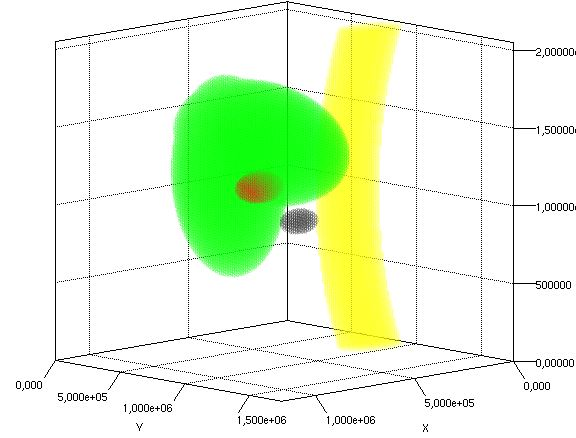
\includegraphics[width=.7\textwidth]{pictures/body}
\caption{Example body with tumor}
\label{model:body}
\end{figure}

Inside the body, the seeds are positioned randomly within the tumor voxels. When eradiating into the surrounding tissue, the seeds influence overlap and form a superposition. Hence, the dosis in a voxel is calculated as a sum of each seed by evaluating the dose-function up to a fixed limit, where the influence gets negligible (see chapter \ref{dose_function}).

\subsection{Evaluation criteria}
	Reflecting the multicriteria nature of the problem, several measurements are considered for treatment evaluation.
	\begin{description}
		\item[Coverage (CO)]~\\
			The fraction of PTV volume that receives at least the prescription dose. Therefore, the CO is always smaller than or equal to 1 and becomes 1 ideally.
		\item[Homogeneity (HI)]~\\
			The upper PTV bound divided by lower PTV bound. Therefore, the HI is always greater than or equal to 1 and becomes 1 ideally.
		\item[Conformality Index (CI)]~\\
			The volume receiving at least the prescription dose divided by the PTV volume receiving at least the prescription dose. Therefore, the CI is always greater than or equal to 1 and becomes 1 ideally.
		\item[Minimum, maximum and average values]~\\
			The extreme and average values per volume of interest.
		\item[Dose Volume Histogram (DVH)]~\\
			A two-dimensional representation of the dose distribution. For a given dose, the cumulative DVH shows the fraction of a volume that is exposed to at least the given dose. Figure \ref{fig:evalCritDVH} shows a typical DVH.
			\begin{figure}[ht]
				\centering
				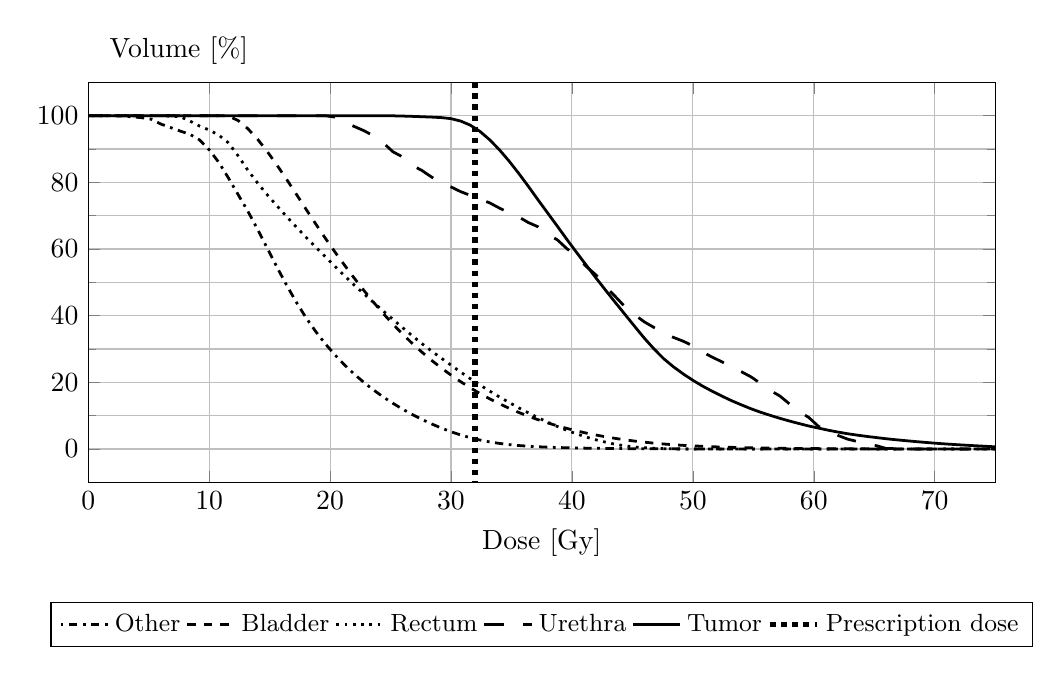
\begin{tikzpicture}
  \begin{axis}[
  	name=one,
  	width=0.95 \columnwidth,
  	height=2.0in, 
  	scale only axis,
  	xtick={0,10,...,80},
  	ytick={0,20,...,100},
  	minor ytick={10,30,...,90},
  	legend style={anchor=north,at={(0.5,-0.30)},font=\small},
  	legend columns=6,
    xmin=0,
    xmax=75,
  	ymax = 110,
  	ymin = -10,
    grid=both,
    y label style={at={(axis description cs:0.1,1.02)},anchor=south,rotate=270},
    ylabel = {Volume [\%]},
    xlabel = {Dose [Gy]}
  	]
\addplot [color=black,dash pattern=on 1pt off 2pt on 3pt off 2pt,line width=1.0pt]
	table[row sep=crcr]{-0.4 100.0 \\
0.4 100.0 \\
1.2000000000000002 100.0 \\
2.0 99.98287739703625 \\
2.8000000000000003 99.89388087384742 \\
3.6 99.66780099639195 \\
4.4 99.3960950212187 \\
5.200000000000001 98.94434538853442 \\
6.000000000000001 97.49907466172606 \\
6.800000000000001 96.45531359483411 \\
7.6000000000000005 95.39555776110176 \\
8.4 94.43371860898844 \\
9.200000000000001 92.75437062130442 \\
10.000000000000002 89.79308308358598 \\
10.8 85.99934995627072 \\
11.600000000000001 81.29586319963008 \\
12.4 76.31462116497269 \\
13.200000000000001 71.3547054861025 \\
14.000000000000002 65.95800963582172 \\
14.8 60.29781025490123 \\
15.600000000000001 54.63248434614727 \\
16.4 49.19733953711555 \\
17.2 44.105672092925495 \\
18.0 39.46965044257315 \\
18.8 35.32290460864599 \\
19.6 31.593458140362284 \\
20.4 28.25239742074132 \\
21.2 25.217800535004447 \\
22.0 22.475313205217986 \\
22.8 19.97059423634729 \\
23.6 17.695851306085498 \\
24.4 15.612020272341665 \\
25.2 13.71202652670562 \\
26.0 11.953730010386344 \\
26.8 10.351382470760848 \\
27.6 8.874532332498392 \\
28.4 7.526665634525728 \\
29.2 6.292300262785816 \\
30.0 5.18763604523238 \\
30.8 4.216774204132187 \\
31.6 3.3853539201020384 \\
32.4 2.688453726421817 \\
33.2 2.125458439751507 \\
34.0 1.6833466793941265 \\
34.8 1.3195682643319775 \\
35.6 1.0445813113453135 \\
36.4 0.8426986452637546 \\
37.2 0.6791624073764584 \\
38.0 0.5531523532300714 \\
38.800000000000004 0.45236481602429557 \\
39.6 0.3745441235124098 \\
40.4 0.3070790172241082 \\
41.2 0.25663398334288573 \\
42.0 0.21141800785179002 \\
42.800000000000004 0.17696774081095518 \\
43.6 0.1472338793769013 \\
44.4 0.11996075130290705 \\
45.2 0.10078753720577575 \\
46.0 0.08222950644865935 \\
46.800000000000004 0.06797775907164733 \\
47.6 0.05618674505469492 \\
48.4 0.0469589949544713 \\
49.2 0.03855148930760089 \\
50.0 0.03219459479411351 \\
50.800000000000004 0.026760475290648494 \\
51.6 0.022249130797205835 \\
52.4 0.018455500200447235 \\
53.2 0.015482114057041849 \\
54.0 0.013431502923658823 \\
54.800000000000004 0.010765708450260888 \\
55.6 0.008920158430216164 \\
56.4 0.0076897917501863484 \\
57.2 0.006869547296833137 \\
58.0 0.005946772286810776 \\
58.800000000000004 0.005126527833457566 \\
59.6 0.004921466720119263 \\
60.4 0.004101222266766053 \\
61.2 0.0035885694834202966 \\
62.0 0.003178447256743691 \\
62.800000000000004 0.0026657944733979345 \\
63.6 0.0023582028033904807 \\
64.4 0.0020506111333830268 \\
65.2 0.001845550020044724 \\
66.00000000000001 0.00153795835003727 \\
66.80000000000001 0.0014354277933681188 \\
67.60000000000001 0.0012303666800298162 \\
68.4 0.0011278361233606647 \\
69.2 0.0010253055666915134 \\
70.00000000000001 9.22775010022362E-4 \\
70.80000000000001 9.22775010022362E-4 \\
71.60000000000001 6.15183340014908E-4 \\
72.4 4.101222266766053E-4 \\
73.2 4.101222266766053E-4 \\
74.00000000000001 2.0506111333830264E-4 \\
74.80000000000001 2.0506111333830264E-4 \\
75.60000000000001 2.0506111333830264E-4 \\
76.4 2.0506111333830264E-4 \\
77.20000000000002 0.0 \\
78.00000000000001 0.0 \\
78.80000000000001 0.0 \\
	};
\addlegendentry{Other};

\addplot [color=black,dashed,line width=1.0pt]
	table[row sep=crcr]{-0.4 99.99999999999997 \\
0.4 99.99999999999997 \\
1.2000000000000002 99.99999999999997 \\
2.0 99.99999999999997 \\
2.8000000000000003 99.99999999999997 \\
3.6 99.99999999999997 \\
4.4 99.99999999999997 \\
5.200000000000001 99.99999999999997 \\
6.000000000000001 99.99999999999997 \\
6.800000000000001 99.99999999999997 \\
7.6000000000000005 99.99999999999997 \\
8.4 99.99999999999997 \\
9.200000000000001 99.99999999999997 \\
10.000000000000002 99.99999999999997 \\
10.8 99.99999999999997 \\
11.600000000000001 99.8921449992108 \\
12.4 98.53606566001997 \\
13.200000000000001 96.1080128373757 \\
14.000000000000002 92.97364129005102 \\
14.8 89.28684168990371 \\
15.600000000000001 85.22123428210658 \\
16.4 80.9491240069448 \\
17.2 76.51523123059924 \\
18.0 72.02083442942073 \\
18.8 67.60272531172726 \\
19.6 63.28326406060925 \\
20.4 59.125585310675014 \\
21.2 55.13626558636292 \\
22.0 51.27321513126743 \\
22.8 47.562740043142 \\
23.6 44.007470931761986 \\
24.4 40.642921029094545 \\
25.2 37.45330667648761 \\
26.0 34.483348240122055 \\
26.8 31.6646498658389 \\
27.6 29.048508444257376 \\
28.4 26.583627084758245 \\
29.2 24.317356763297727 \\
30.0 22.1734097963908 \\
30.8 20.19782185510601 \\
31.6 18.361656231914555 \\
32.4 16.64912926816436 \\
33.2 15.049718524754036 \\
34.0 13.587099489661703 \\
34.8 12.232335455358552 \\
35.6 10.980165202293891 \\
36.4 9.826642815804703 \\
37.2 8.795443783869102 \\
38.0 7.8300099963171474 \\
38.800000000000004 6.948755721576262 \\
39.6 6.1635187036355035 \\
40.4 5.432209186089336 \\
41.2 4.769295522702163 \\
42.0 4.185300152575367 \\
42.800000000000004 3.6565475877308358 \\
43.6 3.1817225232808966 \\
44.4 2.748987215236492 \\
45.2 2.3741253222496974 \\
46.0 2.0466144052191297 \\
46.800000000000004 1.7519861103803862 \\
47.6 1.5033934866101963 \\
48.4 1.2811069605934655 \\
49.2 1.0969642763192509 \\
50.0 0.9457042142368601 \\
50.800000000000004 0.8062818961435262 \\
51.6 0.6865891513652865 \\
52.4 0.5826800652391225 \\
53.2 0.5037617719787448 \\
54.0 0.4287893933813859 \\
54.800000000000004 0.36170884411006476 \\
55.6 0.3077813437154733 \\
56.4 0.2722681117483033 \\
57.2 0.22754774556742255 \\
58.0 0.18940390382490663 \\
58.800000000000004 0.16046719629610143 \\
59.6 0.13810701320566107 \\
60.4 0.11574683011522072 \\
61.2 0.10390908612616405 \\
62.0 0.07760298837270478 \\
62.800000000000004 0.06444993949597516 \\
63.6 0.055242805282264426 \\
64.4 0.043405061293207765 \\
65.2 0.03288262219182407 \\
66.00000000000001 0.03025201241647814 \\
66.80000000000001 0.022360183090440362 \\
67.60000000000001 0.017098963539748515 \\
68.4 0.01446835376440259 \\
69.2 0.010522439101383702 \\
70.00000000000001 0.007891829326037774 \\
70.80000000000001 0.006576524438364813 \\
71.60000000000001 0.005261219550691851 \\
72.4 0.0026306097753459254 \\
73.2 0.0013153048876729627 \\
74.00000000000001 0.0013153048876729627 \\
74.80000000000001 0.0 \\
75.60000000000001 0.0 \\
76.4 0.0 \\
77.20000000000002 0.0 \\
78.00000000000001 0.0 \\
78.80000000000001 0.0 \\
	};
\addlegendentry{Bladder};

\addplot [color=black,dotted,line width=1.0pt]
	table[row sep=crcr]{-0.4 100.0 \\
0.4 100.0 \\
1.2000000000000002 100.0 \\
2.0 100.0 \\
2.8000000000000003 100.0 \\
3.6 100.0 \\
4.4 100.0 \\
5.200000000000001 100.0 \\
6.000000000000001 100.0 \\
6.800000000000001 99.84689971931616 \\
7.6000000000000005 99.73207450880328 \\
8.4 98.40520540954326 \\
9.200000000000001 96.89546653057754 \\
10.000000000000002 95.70681296249045 \\
10.8 94.15879901335376 \\
11.600000000000001 91.84528366079783 \\
12.4 87.93697371778515 \\
13.200000000000001 83.65229225142468 \\
14.000000000000002 79.84392276941396 \\
14.8 76.29497320745088 \\
15.600000000000001 73.01394913668453 \\
16.4 69.75418899379093 \\
17.2 66.6390235604321 \\
18.0 63.5791443395424 \\
18.8 60.64046950752744 \\
19.6 57.71880581781067 \\
20.4 54.81840605596666 \\
21.2 51.95415497150634 \\
22.0 49.16858042017521 \\
22.8 46.555243684613416 \\
23.6 43.95041252020073 \\
24.4 41.41575231776813 \\
25.2 38.88959768648464 \\
26.0 36.395338947010295 \\
26.8 33.96912477672876 \\
27.6 31.615207961214598 \\
28.4 29.369737177851498 \\
29.2 27.251849961724933 \\
30.0 25.161605851832952 \\
30.8 23.084120098664627 \\
31.6 21.087437271412774 \\
32.4 19.199200476311983 \\
33.2 17.376881857616738 \\
34.0 15.631113379263418 \\
34.8 13.981032576337501 \\
35.6 12.360721272433445 \\
36.4 10.853108786254998 \\
37.2 9.388024155822064 \\
38.0 8.03563834311474 \\
38.800000000000004 6.757676277962066 \\
39.6 5.579654673811347 \\
40.4 4.507952709024411 \\
41.2 3.5723398826231185 \\
42.0 2.7409203027983327 \\
42.800000000000004 2.034957897422812 \\
43.6 1.4012928468146635 \\
44.4 0.9419920047631197 \\
45.2 0.5975163732244619 \\
46.0 0.3806243089223441 \\
46.800000000000004 0.21901845708939355 \\
47.6 0.1041932465765076 \\
48.4 0.042527855745513314 \\
49.2 0.012758356723653993 \\
50.0 0.0 \\
50.800000000000004 0.0 \\
51.6 0.0 \\
52.4 0.0 \\
53.2 0.0 \\
54.0 0.0 \\
54.800000000000004 0.0 \\
55.6 0.0 \\
56.4 0.0 \\
57.2 0.0 \\
58.0 0.0 \\
58.800000000000004 0.0 \\
59.6 0.0 \\
60.4 0.0 \\
61.2 0.0 \\
62.0 0.0 \\
62.800000000000004 0.0 \\
63.6 0.0 \\
64.4 0.0 \\
65.2 0.0 \\
66.00000000000001 0.0 \\
66.80000000000001 0.0 \\
67.60000000000001 0.0 \\
68.4 0.0 \\
69.2 0.0 \\
70.00000000000001 0.0 \\
70.80000000000001 0.0 \\
71.60000000000001 0.0 \\
72.4 0.0 \\
73.2 0.0 \\
74.00000000000001 0.0 \\
74.80000000000001 0.0 \\
75.60000000000001 0.0 \\
76.4 0.0 \\
77.20000000000002 0.0 \\
78.00000000000001 0.0 \\
78.80000000000001 0.0 \\
	};
	\addlegendentry{Rectum};

\addplot [color=black,dash pattern=on 7pt off 7pt,line width=1.0pt]
	table[row sep=crcr]{-0.4 99.99999999999999 \\
0.4 99.99999999999999 \\
1.2000000000000002 99.99999999999999 \\
2.0 99.99999999999999 \\
2.8000000000000003 99.99999999999999 \\
3.6 99.99999999999999 \\
4.4 99.99999999999999 \\
5.200000000000001 99.99999999999999 \\
6.000000000000001 99.99999999999999 \\
6.800000000000001 99.99999999999999 \\
7.6000000000000005 99.99999999999999 \\
8.4 99.99999999999999 \\
9.200000000000001 99.99999999999999 \\
10.000000000000002 99.99999999999999 \\
10.8 99.99999999999999 \\
11.600000000000001 99.99999999999999 \\
12.4 99.99999999999999 \\
13.200000000000001 99.99999999999999 \\
14.000000000000002 99.99999999999999 \\
14.8 99.99999999999999 \\
15.600000000000001 99.99999999999999 \\
16.4 99.99999999999999 \\
17.2 99.99999999999999 \\
18.0 99.99999999999999 \\
18.8 99.99999999999999 \\
19.6 99.99999999999999 \\
20.4 99.57805907172995 \\
21.2 98.17158931082982 \\
22.0 96.76511954992966 \\
22.8 95.49929676511954 \\
23.6 93.95218002812939 \\
24.4 91.84247538677918 \\
25.2 89.17018284106892 \\
26.0 87.62306610407877 \\
26.8 85.09142053445852 \\
27.6 83.54430379746837 \\
28.4 81.57524613220816 \\
29.2 79.88748241912799 \\
30.0 78.62165963431788 \\
30.8 77.21518987341773 \\
31.6 76.09001406469761 \\
32.4 74.96483825597751 \\
33.2 73.8396624472574 \\
34.0 72.29254571026725 \\
34.8 70.8860759493671 \\
35.6 69.62025316455697 \\
36.4 67.93248945147681 \\
37.2 66.66666666666669 \\
38.0 64.41631504922645 \\
38.800000000000004 62.72855133614629 \\
39.6 60.056258790436026 \\
40.4 57.805907172995795 \\
41.2 54.711673699015485 \\
42.0 52.180028129395225 \\
42.800000000000004 48.66385372714488 \\
43.6 45.71026722925458 \\
44.4 42.61603375527427 \\
45.2 40.22503516174403 \\
46.0 38.11533052039382 \\
46.800000000000004 36.42756680731365 \\
47.6 34.73980309423348 \\
48.4 33.473980309423354 \\
49.2 32.34880450070324 \\
50.0 30.942334739803094 \\
50.800000000000004 29.11392405063291 \\
51.6 27.566807313642755 \\
52.4 26.160337552742615 \\
53.2 24.613220815752456 \\
54.0 23.206751054852315 \\
54.800000000000004 21.65963431786216 \\
55.6 19.690576652601965 \\
56.4 17.580872011251756 \\
57.2 15.893108298171587 \\
58.0 13.502109704641349 \\
58.800000000000004 11.251758087201125 \\
59.6 9.423347398030941 \\
60.4 6.751054852320674 \\
61.2 5.9071729957805905 \\
62.0 4.0787623066104075 \\
62.800000000000004 2.9535864978902953 \\
63.6 2.250351617440225 \\
64.4 1.4064697609001406 \\
65.2 0.9845288326300984 \\
66.00000000000001 0.14064697609001406 \\
66.80000000000001 0.14064697609001406 \\
67.60000000000001 0.0 \\
68.4 0.0 \\
69.2 0.0 \\
70.00000000000001 0.0 \\
70.80000000000001 0.0 \\
71.60000000000001 0.0 \\
72.4 0.0 \\
73.2 0.0 \\
74.00000000000001 0.0 \\
74.80000000000001 0.0 \\
75.60000000000001 0.0 \\
76.4 0.0 \\
77.20000000000002 0.0 \\
78.00000000000001 0.0 \\
78.80000000000001 0.0 \\
	};
\addlegendentry{Urethra};

\addplot [color=black,solid,line width=1.0pt]
	table[row sep=crcr]{-0.4 100.00000000000003 \\
0.4 100.00000000000003 \\
1.2000000000000002 100.00000000000003 \\
2.0 100.00000000000003 \\
2.8000000000000003 100.00000000000003 \\
3.6 100.00000000000003 \\
4.4 100.00000000000003 \\
5.200000000000001 100.00000000000003 \\
6.000000000000001 100.00000000000003 \\
6.800000000000001 100.00000000000003 \\
7.6000000000000005 100.00000000000003 \\
8.4 100.00000000000003 \\
9.200000000000001 100.00000000000003 \\
10.000000000000002 100.00000000000003 \\
10.8 100.00000000000003 \\
11.600000000000001 100.00000000000003 \\
12.4 100.00000000000003 \\
13.200000000000001 100.00000000000003 \\
14.000000000000002 100.00000000000003 \\
14.8 100.00000000000003 \\
15.600000000000001 100.00000000000003 \\
16.4 100.00000000000003 \\
17.2 100.00000000000003 \\
18.0 100.00000000000003 \\
18.8 100.00000000000003 \\
19.6 100.00000000000003 \\
20.4 100.00000000000003 \\
21.2 100.00000000000003 \\
22.0 100.00000000000003 \\
22.8 100.00000000000003 \\
23.6 100.00000000000003 \\
24.4 99.99358639582934 \\
25.2 99.95510477080528 \\
26.0 99.88638758326233 \\
26.8 99.7947646665384 \\
27.6 99.6875658539714 \\
28.4 99.5730372080665 \\
29.2 99.42369185380649 \\
30.0 99.11125770777788 \\
30.8 98.38743666565883 \\
31.6 97.15235974822023 \\
32.4 95.26126274703829 \\
33.2 92.77095187048184 \\
34.0 89.77671495194379 \\
34.8 86.40041047066693 \\
35.6 82.69243103084943 \\
36.4 78.7828811742393 \\
37.2 74.73406448420879 \\
38.0 70.772289565066 \\
38.800000000000004 66.81143087509047 \\
39.6 62.79468220591333 \\
40.4 58.90803807848418 \\
41.2 55.072702784420436 \\
42.0 51.27035174037729 \\
42.800000000000004 47.555042467221895 \\
43.6 43.911199069111156 \\
44.4 40.315915816864106 \\
45.2 36.725213710453254 \\
46.0 33.19589895824743 \\
46.800000000000004 29.9762696645685 \\
47.6 27.052582391907865 \\
48.4 24.648397057071918 \\
49.2 22.53465636825083 \\
50.0 20.616072492051714 \\
50.800000000000004 18.886231824303895 \\
51.6 17.32222863582639 \\
52.4 15.87641900992276 \\
53.2 14.498410342394838 \\
54.0 13.266082112457966 \\
54.800000000000004 12.086895174220976 \\
55.6 11.028650486059572 \\
56.4 10.096845422977195 \\
57.2 9.205354443253347 \\
58.0 8.387161796908643 \\
58.800000000000004 7.619361754762101 \\
59.6 6.890959566806849 \\
60.4 6.265175045582401 \\
61.2 5.637558066023473 \\
62.0 5.081406961509213 \\
62.800000000000004 4.583894523698268 \\
63.6 4.1578479609319885 \\
64.4 3.7721154815242386 \\
65.2 3.4211997104715826 \\
66.00000000000001 3.0757813144223634 \\
66.80000000000001 2.7761743767351086 \\
67.60000000000001 2.5022218557305553 \\
68.4 2.238347855565634 \\
69.2 1.9918822095782596 \\
70.00000000000001 1.7564113135977568 \\
70.80000000000001 1.543846146798237 \\
71.60000000000001 1.3532704800124604 \\
72.4 1.180103167404231 \\
73.2 1.0151819173011551 \\
74.00000000000001 0.854841813034276 \\
74.80000000000001 0.6990828546035933 \\
75.60000000000001 0.5634809378521755 \\
76.4 0.43062770860247557 \\
77.20000000000002 0.3005231668544936 \\
78.00000000000001 0.18874320845129783 \\
78.80000000000001 0.09345537505840962 \\
	};
\addlegendentry{Tumor};
  \addplot [color=black,dotted,line width=2.0pt]
  	table[row sep=crcr]{32.0 110.0 \\
  	32.0 -10.0 \\
  	};
  	 \addlegendentry{Prescription dose};
  \addplot [color=black,dotted,line width=2.0pt]
  	table[row sep=crcr]{32.0 110.0 \\
  	32.0 -10.0 \\
  	};
\end{axis}

    
\end{tikzpicture} 
				\caption{A cumulative dose volume histogram}
				\label{fig:evalCritDVH}
			\end{figure}
			


\end{description}

\section{Dose-Function}\label{dose_function}
The dose-distribution within the patient's body is the accumulation of all the radiation-seeds. Therefore, it is mandatory to know the radiation intensity of each seed. Equation \eqref{eq:dosefunction} shows the general approach to approximate the dose intensity function, whilst \eqref{eq:dosefunction2} is showing the used implementation of that equation.
\begin{equation}
\label{eq:dosefunction}
\dot{D}(r,\theta_{0})= S_{k}\Lambda \frac{G_{L}(r,\theta_{0})}{G_{L}(r_{0},\theta_{0})} g_{L}(r) F(r_{0},\theta_{0})
\end{equation}
\begin{equation}
\label{eq:dosefunction2}
\Rightarrow \ \dot{D}(r,\theta_{0})= S_{k}\Lambda \frac{G_{L}(r,\theta_{0})}{G_{L}(r_{0},\theta_{0})} g_{L}(r) \cdot 1
\end{equation}
\\
The following section will describe the used parameters:
\begin{description}
\item[Air-Kerma-Strength $S_{k}$]~\\
The $S_{k}$ describes the \textbf{k}inetic \textbf{e}nergy \textbf{r}eleased per unit \textbf{ma}ss called kerma. It is measured in $U$ ($1\ U =1 \ \frac{cGy \cdot m^{2}}{h} $)   
\item[Dose Rate Constant $\Lambda$]~\\
The dose rate constant is defined as the ratio of the dose rate at reference point $ P(r_{0},\theta_{0})  $ and the air-kerma-strength $S_{k}$. Therefore $ \Lambda \ = \ \frac{\dot{D}(r_{0},\theta_{0})}{S_{k}} $.



\item[Dose Function $g_{L}(r)$]~\\
The dose function describes the dose intensity depending on the radial distance.


\item[Two dimensional anisotropy function $ F(r_{0},\theta_{0})$]~\\
The anisotropy resolves issues due to the fact that the dose distribution isn't rotation invariant. Therefore, the dose intensity is different for different angles.


\item[Geometry Function $G_{L}(r_{0},\theta_{0})$ ]~\\
Due to scatter and attenuation, an estimation of the dose distribution with point sources is less precise then an estimation with a line source. Therefore, a line source model is used. Figure \ref{fig:geometry} gives an overview of the geometry of the model.

\begin{figure}[hbtp]


\centering
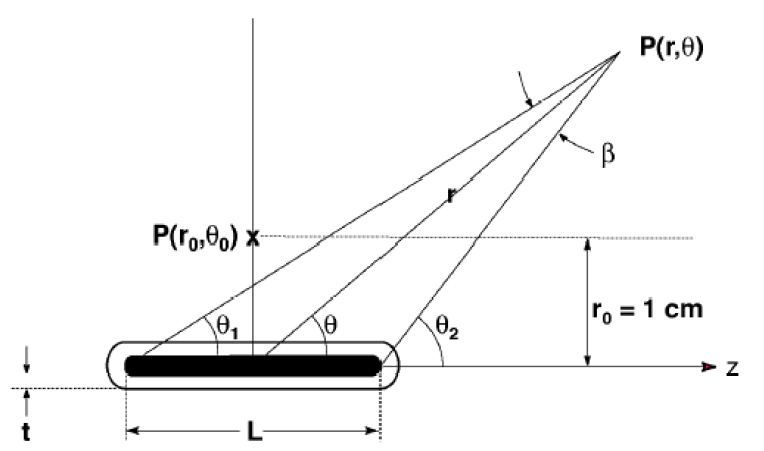
\includegraphics[width=0.7\textwidth]{pictures/geometry}
\caption{Geometry of a line source}
\label{fig:geometry}	
\end{figure}
\end{description}

Figure \ref{fig:doseplot} shows the plotted dose function. It is easily seen that the curve has a significant steep slope. Hence, it should be discussed, for which radii the given function should be evaluated.

\begin{figure}[htbp]

\centering
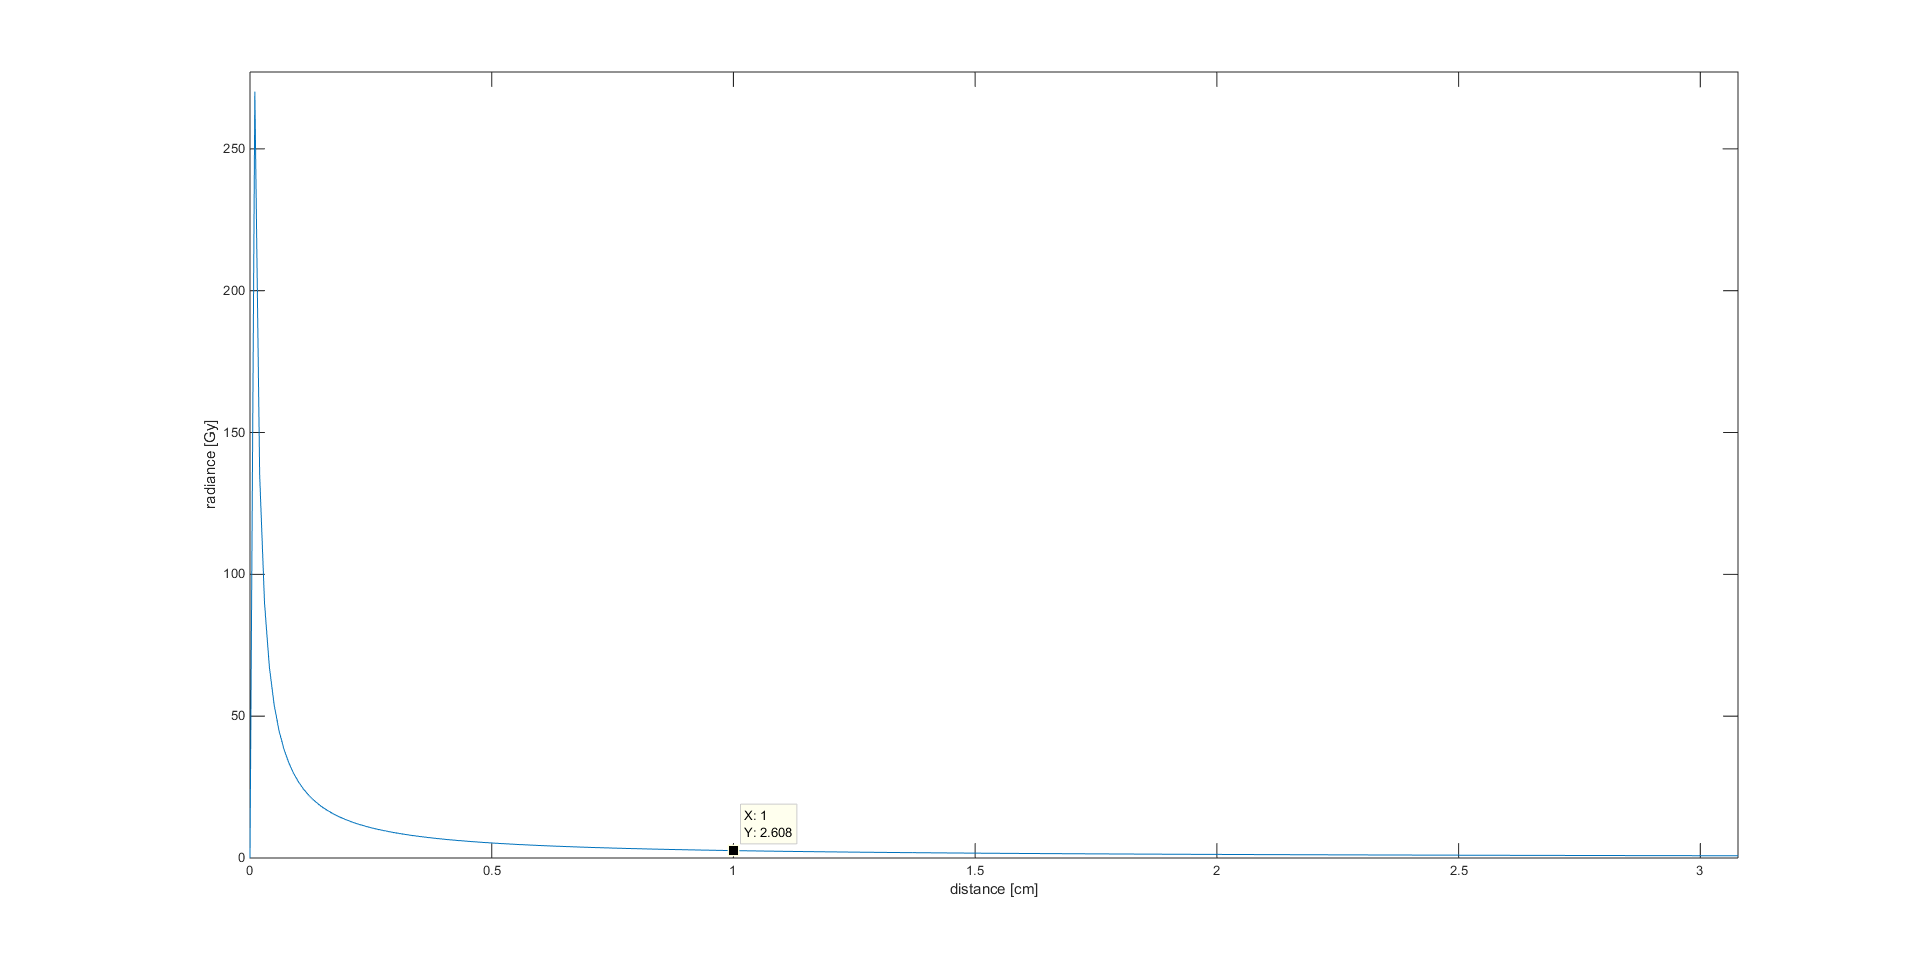
\includegraphics[width=0.9\textwidth]{pictures/dosefunction}
\caption{Dose-Function Plot}
\label{fig:doseplot}
\end{figure}
\section{Genetic Algorithm}
\label{sec:genalg}

Genetic algorithm  or evolutionary algorithm \cite{genpro} describes a search procedure which belongs to the category of local searches\cite{aima}. Local search algorithms are used when the path to your solution is irrelavant (unlike e.g. breadth first search). The idea of the genetic algorithm is to find the best solution in a solution space by adapting the procedure of genetic reproduction to the problem. \\ 
The algorithm consists mainly of three components:

\begin{description}
\item[Individual]~\\
\label{indiv}
An individual contains one possible solution for the problem. It could be seen as the interface between the problem and the algorithm.  It is forced to reproduce itself with other individuals so the solution might improve. The key is to find an efficient encoding for your problem.
\item[Population]~\\
\label{pop}
The collection of all individuals is called population. The population provides the gene pool. Every individual shall reproduce it's gene with another one out of the population. 
\item[Fitness-Function]~\\
\label{fifu}
The fitness-function is a heuristic which is used to evaluate the fitness value of an individual. The fitness value indicates the quality of a solution contained by the individual. Further on, the fitness value is used to select the best individuals for reproduction.
\end{description} 

The genetic algorithm is an iterative algorithm. Each iteration consists of four steps, which are described in the following:

\begin{description}
\item[1. Elitism]~\\
In the elitism step, a specific number of the best individuals are taken into the next iteration without further reproduction or other actions. 
\item[2. Selection]~\\
During the selection phase, each individual gets selected with a probabilty which is proportional to its fitnessvalue.\\
$P_{selection_{i}}= \tfrac{fitness_{i}}{\sum_{j}^I fitness_{j}}$, where $I$ is the population size and $i$ the specific index for an individual.
\item[3. Crossover]~\\
During the crossover step the previously selected individuals are taken pairwise to exchange their solution by using the one point crossover. One point crossover cuts the gene in two parts at a randomly chosen point and swaps one half of each gene.



\item[4. Mutation]~\\
In the end, each individual changes randomly some parts of its solution by a given probability.
\end{description}

\subsection{Implementation}
\label{subsec:impl}

The individual is implemented as a $n$-dimensional vector of dwell times, where $n$ denotes the number of seeds. Equation \eqref{eq:individual} shows one individual for $n $ seeds.
 \begin{equation}
 \label{eq:individual}
 Individual \ \ i := \begin{pmatrix}
 t_{0} \\ \vdots \\ t_{n-1} 	
\end{pmatrix}   
\end{equation} 
 
 The population is the accumulation of all individuals (see \ref{pop}) $k$ denotes the number of individuals.
\begin{equation}
 \label{eq:population}
 Population \ \ p := \begin{pmatrix}
 i_{0} \\ \vdots \\ i_{k-1} 	
\end{pmatrix}   
 \end{equation}
 
 The fitness-function calculates the squared difference between the goal dose and the current dose within the whole body.
 \begin{equation}
 f(individual) = \sum_{body}(GD-CD)^2
 \end{equation}
 For further adjustment and prioritisation the fitness-function is extended by a weight factor, which holds a specific weight for any body type (i.e. tumor, liver, spine).
 \begin{equation}
 \label{eq:fifu}
 f(individual) = \sum_{body}w_{bodytype}(GD-CD)^2
 \end{equation}

\subsubsection{Optimization}
\label{subsubsec:optimization}
The calculation of the fitness-function, as described in equation \eqref{eq:fifu}, is shown in algorithm \ref{alg:fifu}. It is easily seen that it iterates over every voxel in the body. This results in a very high computational complexity and runtime. To improve the performance of the algorithm, three different optimization approaches are introduced. \\

\begin{algorithm}[H]
\label{alg:fifu}
 $temp=0$\;
 \For{x=0; x $\textless$ body.xDim; x++}{
 	\For{y=0; y $\textless$ body.yDim; y++}{
 		\For{z=0; z $\textless$ body.zDim; z++}{
 			\For{j=0; j $\textless$ numberOfSeeds; j++} {
				 	$temp\ \ = temp+  w_{bodytype}(GD-CD)^2$\;		
 			}
  		}
  	}
  }
 $fitnessvalue = \sqrt{temp}$\;
 \Return{fitnessvalue}\;
 \caption{Calculation of the fitnessvalue}
 
 \end{algorithm}


\paragraph{Scaling}
\label{para:scaling}
~\\
This strategy evaluates not every single voxel in the body. Only every n$th$ voxel is evaluated. Algorithm \ref{alg:scalefif} shows the implementation of scaling. \\

\paragraph{Treatment Range}
\label{para:treatment range}
As it is shown in chapter \ref{dose_function}, the distribution of the radiation decreases exponentially with increasing distance. This effect could be used to reduce the number of voxel being evaluated, as the influence of voxels relatively far away is negligibly small. Algorithm \ref{alg:scalefif} shows how that information is used. The region of interest (ROI) denotes the treatment range. \\



\begin{algorithm}[H]
\label{alg:scalefif}

 \For{y=y-roi.min; y $\textless$ y-rio.max; y$\leftarrow$y+Scalefactor}{
 		\For{z=z-roi.min; z $\textless$ z-rio.max; z$\leftarrow$z+Scalefactor}{
 			\For{j=0; j $\textless$ numberOfSeeds; j++} {
				 	$temp\ \ = temp+  w_{bodytype}(GD-CD)^2$\;		
 			}
  		}
  	}
\caption{Optimised fitness-function}
\end{algorithm} 






\paragraph{Multithreading}
\label{para:multithreading}
~\\ 
The multithreading approach seperates the three-dimensional body into two-dimensional planes. Each plane is then processed in an own thread. Algorithm \ref{alg:multithread} demonstrates this approach.\\

 \begin{algorithm}[H]
 \label{alg:multithread}
 \SetKwFunction{cb}{CalculateBounds}
 \SetKwFunction{thread}{ThreadedFitnessFunction}

 \emph{x-roi,y-roi,z-roi $\leftarrow$} \cb{body}  \;
 \For{x-roi}{
 	\thread{x,y-roi,z-roi}
 }
 \caption{Multithreaded Fitness-Function}
 \end{algorithm} 

\subsubsection{Stoping Criterion}
\label{subsubsec: stopcrit}
One of the challenges for the genetic algorithm is to decide when and how the algorithm should terminate. It is difficult to determine how close the current iteration is to the optimal solution. The approach used in this implementation calculates the difference between the current fitness-value and the fitness-value of the previous iteration. If the absolute value of this difference is less or equal to a small boundary value, a counter is incremented. If this counter is incremented five times in a row, the algorithm terminates. \\ 
This procedure shall ensure that small fluctuations, that can occur due to mutations within the individuals, will have no effect on the termination. \\


\begin{algorithm}[H]
\SetKwFunction{iter}{GeneticAlgIteration}
$individualOld,currentIndividual \leftarrow 0$\;
$stop \leftarrow false$\;
$counter \leftarrow 0$\;
\While{! stop} {
 \tcc{Returns the best fitness value from the current iteration}
 	
	$currentIndividual \leftarrow $\iter{}\;
	
	\If{$\left|individualOld-currentIndividual \right| \ \ \textless \ \ 1$} {
		\emph{counter++}
	} 
	\If{$counter \geq 5$} {
		$done \leftarrow true$
	}  
	$individualOld \leftarrow currentIndividual $
	
	
	
	
	}
	 

\caption{Stop-Criterion}
\end{algorithm}  

\newpage
\subsubsection{Parameters}
The implemented algorithm has a set of parameters, which is used to adjust its outcome. The usage and the influence of those values are described and discussed in the following.

\paragraph{Weights}~\\
The fitness-function as described in \ref{fifu} uses individual weighting factors for each body type.  Nonetheless, every tissue type can be weighted with an individual coefficent. 

\paragraph{Probabilities} ~\\ 
There are two important probabilities within the algorithm. The first one is the crossover rate. It describes how likely it is for two individuals to reproduce. The second one is the mutation rate. It describes, analogous to the crossover rate, the probability for an individual to perform a mutation. 

\paragraph{Scaling and Accuracy}~\\
The fitness-function for the given optimization problem has very high computational complexity. Hence, two scaling parameters are introduced to achieve shorter runtimes. The challenge here is to find a compromise between good accuracy for the optimization and practicable runtimes.\\ The first parameter is the treatment range. It chooses the range around the PTV which shall be evaluated by the algorithm. The second parameter is a simple scaling value which defines that just every  n$th$ voxel is evaluated within the treatment range.



\subsubsection{Results}


\paragraph{Weights}
It seems hard to examine a specific sets of weights, that is applicable to any type of patient. The experiment has shown, that a higher weighted treatment has a much higher runtime and the convergency decreases.  Figure \ref{fig:weights} shows the difference between the goal dose and the actual dose for different weighted distributions.
\begin{figure}[hbtp]
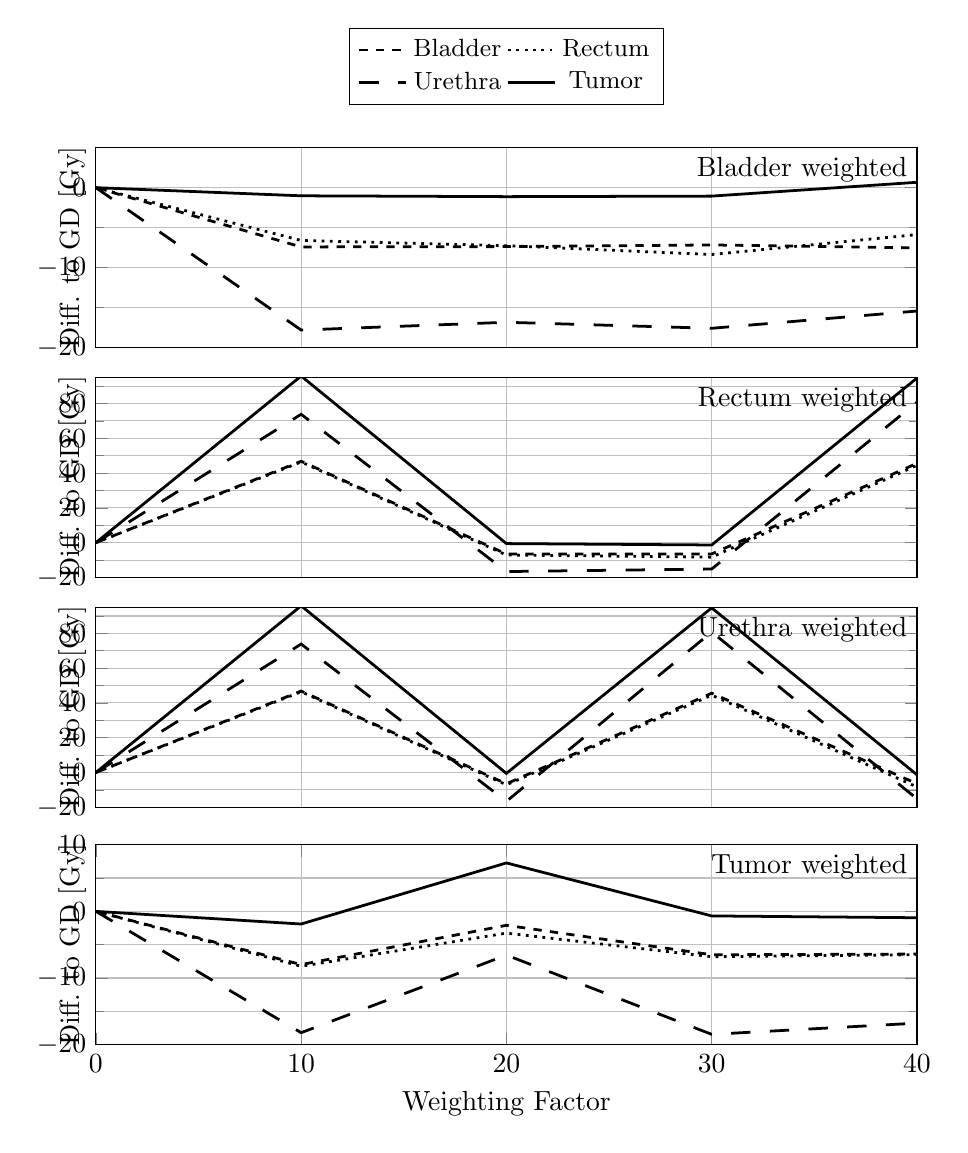
\begin{tikzpicture}
  \begin{axis}[
  	name=one,
  	width=0.86 \columnwidth,
  	height=1.0in, 
  	scale only axis,
  	xmajorticks=false,
  	xtick={0,10,20,30,40},
  	ytick={-20,-10,...,10},
  	minor ytick={-20,-15,...,10},
  	legend style={anchor=north,at={(0.5,1.6)},font=\small},
  	legend columns=2,
    xmin=0,
    xmax=40,
  	ymax = 5,
  	ymin = -20,
    grid=both,
    y label style={at={(axis description cs:0,.5)},anchor=south},
    ylabel = {Diff. to GD [Gy]}
    ]
	\addplot [color=black,dashed,line width=1.0pt]
	table[row sep=crcr]{0 0\\
						10 -7.4061373\\
						20 -7.3660937\\
						30 -7.16107\\
						40 -7.5223036\\	};
	\addlegendentry{Bladder};	
	

	
	\addplot [color=black,dotted,line width=1.0pt]
	table[row sep=crcr]{0 0\\
						10 -6.6003648\\
						20 -7.250544\\
						30 -8.3557603\\
						40 -5.8634733\\ };
	\addlegendentry{Rectum};   
   
    
	
	\addplot [color=black,dash pattern=on 7pt off 7pt,line width=1.0pt]
	table[row sep=crcr]{0 0\\
						10 -17.7968793\\
						20 -16.8252388\\
						30 -17.5772547\\
						40 -15.4201025\\ };
	\addlegendentry{Urethra};
	
	\addplot [color=black,solid,line width=1.0pt]
	table[row sep=crcr]{0 0\\
	 					10 -1.0171151\\
	 					20 -1.1222384\\
				 		30 -1.0559538\\
	 					40  0.6725971\\};
	\addlegendentry{Tumor};					
  \node at (rel axis cs:1,1) [anchor=north east] {Bladder weighted};	
  \end{axis}
  
  \begin{axis}[
  	name=two,
  	width=0.86 \columnwidth,
  	height=1.0in, 
  	scale only axis,
  	at=(one.below south),
    anchor=above north,
  	xmajorticks=false,
  	xtick={0,10,20,30,40},
  	ytick={-20,-0,...,100},
  	minor ytick={-10,0,...,100},
    xmin=0,
    xmax=40,
  	ymax = 95,
  	ymin = -20,
    grid=both,
    y label style={at={(axis description cs:0,.5)},anchor=south},
    ylabel = {Diff. to GD [Gy]}
    ]
	\addplot [color=black,dashed,line width=1.0pt]
	table[row sep=crcr]{0 0\\
						10 46.8163804\\
						20 -6.5099569\\
						30 -6.4596163\\
						40 45.5999754\\ };

	%\addlegendentry{Bladder};	
	
	\addplot [color=black,dotted,line width=1.0pt]
	table[row sep=crcr]{0 0\\
						10 46.4315353\\
						20 -7.0846292\\
						30 -8.312817\\
						40 44.4589502\\ };

	%\addlegendentry{Rectum};   
   
    
	
	\addplot [color=black,dash pattern=on 7pt off 7pt,line width=1.0pt]
	table[row sep=crcr]{0 0\\
						10 73.834936\\
						20 -16.600937\\
						30 -15.1440168\\
						40	80.79331\\  };
	%\addlegendentry{Urethra};
	
	\addplot [color=black,solid,line width=1.0pt]
	table[row sep=crcr]{0 0\\
	 					10 95.820661\\
	 					20 -0.5231224\\
	 					30 -1.3135843\\
	 					40	94.652913\\ };
	%\addlegendentry{Tumor};					
  \node at (rel axis cs:1,1) [anchor=north east] {Rectum weighted};	
  \end{axis}
  \begin{axis}[
  	name=three,
  	width=0.86 \columnwidth,
  	height=1.0in, 
  	scale only axis,
  	at=(two.below south),
    anchor=above north,
  	xmajorticks=false,
  	xtick={0,10,20,30,40},
  	ytick={-20,-0,...,100},
  	minor ytick={-10,0,...,100},
  	legend style={anchor=north,at={(0.5,1.3)},font=\small},
  	legend columns=2,
    xmin=0,
    xmax=40,
  	ymax = 95,
  	ymin = -20,
    grid=both,
    y label style={at={(axis description cs:0,.5)},anchor=south},
    ylabel = {Diff. to GD [Gy]}
    ]
	\addplot [color=black,dashed,line width=1.0pt]
	table[row sep=crcr]{0 0\\
						10 46.8163804\\
						20 -6.5099569\\
						30 45.5999754\\
						40 -6.4596163\\ };

	%\addlegendentry{Bladder};	
	
	\addplot [color=black,dotted,line width=1.0pt]
	table[row sep=crcr]{0 0\\
						10 46.4315353\\
						20 -7.0846292\\
						30 44.4589502\\
						40 -8.312817\\ };

	%\addlegendentry{Rectum};   
   
    
	
	\addplot [color=black,dash pattern=on 7pt off 7pt,line width=1.0pt]
	table[row sep=crcr]{0 0\\
						10 73.834936\\
						20 -16.600937\\
						30 80.79331\\
						40 -15.1440168\\ };
	%\addlegendentry{Urethra};
	
	\addplot [color=black,solid,line width=1.0pt]
	table[row sep=crcr]{0 0\\
	 					10 95.820661\\
	 					20 -0.5231224\\
	 					30 94.652913\\
	 					40 -1.3135843\\ };
	%\addlegendentry{Tumor};					
  \node at (rel axis cs:1,1) [anchor=north east] {Urethra weighted};	
  \end{axis}
  \begin{axis}[
  	name=four,
  	width=0.86 \columnwidth,
  	height=1.0in, 
  	scale only axis,
  	at=(three.below south),
    anchor=above north,
  	xmajorticks=true,
  	xtick={0,10,20,30,40},
  	ytick={-20,-10,...,10},
  	minor ytick={-15,-10,...,5},
    xmin=0,
    xmax=40,
  	ymax = 10,
  	ymin = -20,
    grid=both,
    xlabel = {Weighting Factor},
    y label style={at={(axis description cs:0,.5)},anchor=south},
    ylabel = {Diff. to GD [Gy]}
    ]
	\addplot [color=black,dashed,line width=1.0pt]
	table[row sep=crcr]{0 0\\
						10 -7.9814571\\
						20 -2.0920392\\
						30 -6.5044591\\
						40 -6.4056077\\ };

	%\addlegendentry{Bladder};	
	
	\addplot [color=black,dotted,line width=1.0pt]
	table[row sep=crcr]{0 0\\
						10 -8.2390329\\
						20 -3.2641176\\
						30 -6.7960123\\
						40 -6.5058489\\ };

	%\addlegendentry{Rectum};   
   
    
	
	\addplot [color=black,dash pattern=on 7pt off 7pt,line width=1.0pt]
	table[row sep=crcr]{0 0\\
						10 -18.198227\\
						20 -6.5576085\\
						30 -18.4460054\\
						40 -16.7663932\\ };
	%\addlegendentry{Urethra};
	
	\addplot [color=black,solid,line width=1.0pt]
	table[row sep=crcr]{0 0\\
	 					10 -1.8981359\\
	 					20 7.2659238\\
	 					30 -0.6839885\\
	 					40 -0.955956\\ };
	%\addlegendentry{Tumor};					
  \node at (rel axis cs:1,1) [anchor=north east] {Tumor weighted};	
  \end{axis}
  
\end{tikzpicture}
\caption{Difference between the goal dose and the average dose}
\label{fig:weights}
\end{figure}

\newpage
\paragraph{Probabilities} 
The results have shown, that a high mutation rate leads to a very low tumor coverage. Furthermore, the algorithm often doesn't converge, because the changes of the individuals occur too often. A stable state becomes less likely. \\ For the crossover rate the results showed, that the value should be between 0.7 and 0.9.
% Please add the following required packages to your document preamble:
% \usepackage{multirow}
\begin{table}[h]
\label{table:probabilities}
\begin{tabular}{c|ccccc}
\textbf{MR}          & \textbf{CR :}     & 0.3   & 0.5   & 0.7   & 0.9   \\ \hline
\multirow{2}{*}{0.3} & \textbf{CI}       & 1,092 & 1,019 & 1,683 & 1,101 \\
                     & \textbf{Coverage} & 0,778 & 0,387 & 1,000 & 0,770 \\ \hline
\multirow{2}{*}{0.5} & \textbf{CI}       & 1,028 & 1,032 & 1,022 & 1,079 \\
                     & \textbf{Coverage} & 0,360 & 0,410 & 0,395 & 0,403 \\ \hline
\multirow{2}{*}{0.7} & \textbf{CI}       & 1,007 & 1,046 & 1,012 & 1,035 \\
                     & \textbf{Coverage} & 0,281 & 0,316 & 0,011 & 0,341 \\ \hline
\multirow{2}{*}{0.9} & \textbf{CI}       & 1,034 & 1,000 & 1,109 & 1,043 \\
                     & \textbf{Coverage} & 0,256 & 0,001 & 0,736 & 0,273 \\
\end{tabular}
\caption{Mutation rate and coverage for different mutation \& crossover rates}

\end{table}
\subsubsection{Scaling and Accuracy}
The dose distribution of a radioactive seed shows that the dose at a radius of 10 cm is negligible small. So any treatment range higher than 10 cm wouldn't lead to better results. 
\section{Simulated Annealing}
\label{sec:SAIntro}

Simulated Annealing \cite{genpro} describes a Monte Carlo (deterministic runtime) approach to minimization of multivariate functions. The idea of Simulated Annealing has been first proposed in a paper published by Metropolis et al. in 1953. The algorithm in said paper simulated the cooling of solids in a heat bath. This cooling process is known as annealing.

The idea of the Simulated Annealing algorithm is to find the global minimum of a cost function by randomly selecting a valid solution from the set of viable solutions and determining its cost and keeping solutions which are more optimal than the previous iteration's solution. Following the annealing analogy, a less optimal solution can be accepted following a certain transition probability. This serves to prevent falling into local minima. \\ 
The Simulated Annealing algorithm is comprised of

\begin{description}
\item[State]~\\
\label{state}
A state is any viable solution from the set of viable solutions for a problem. It can take be of any type.
\item[Cost Function]~\\
\label{cofu}
The cost function is at the center of the Simulated Annealing algorithm. It determines the quality of a computed state with respect to certain criteria which embody the cost function. Since the cost is what is minmized (or maximized) during the iterative process, the cost function is the function whose global minimum is sought by Simulated Annealing. \\
that maps from the solution space to $\mathbb{R}$ 
\item[Metropolis Function, Metropolis Loop]~\\
\label{metro}
The \emph{Metropolis Function} is the function that determines how states of higher cost than the previous iteration's candidate solution state are handled. The \emph{Metropolis Loop} is the main loop which determines the cost of a candidate solution, compares it to the current best solution, accepts or discards it according to the Metropolis Function, computes a new candidate state and adjusts the annealing schedule.
\item[Annealing Schedule]~\\
\label{anneal}
As Simulated Annealing is modeled on the annealing of solids, the annealing schedule emulates the influence of temperature on the mobility of molecular structures in solids. The further the virtual temperature drops, the less likely a less optimal state is accepted as the current best. The speed of the temperature decrease is called the \emph{annealing schedule}.
\end{description} 

Simulated Annealing is an iterative algorithm. Each iteration consists of four steps, which are described in the following:                                                           

\begin{description}
\item[1. Next candidate state generation step]~\\
This step consists of one operation: a random generation of a state vector or any other data structure to hold the values determining a solution to the optimization problem.
\item[2. Cost calculation step]~\\
This step calculates the cost of the randomly selected solution and stores it as a numerical value for efficent processing. The cost function is called with the candidate state as the argument.
\item[3. Decision step]~\\
The decision step determines if the currently best solution should be overwritten. If the cost of the candidate solution is better than the current best, the candidate solution becomes the current best and the candidate cost becomes the current best as well. \\ If the the candidate cost is lower than the current best, a random number between 0 and 1 (excluding those) is drawn and if that number lies below the value of the Metropolis Function then the current best cost and state are updated regardless. \\ In any other case, the candidate solution is rejected. 
\item[4. Annealing schedule adaptation step]~\\
In this last step of an iteration, the virtual temperature is updated to a new value according to a predefined annealing schedule that determines the rate at wich the annealing temperature is meant to fall. This temperature is used in the next iteration to determine the value of the Metropolis Function.
\end{description} 

\subsection{Implementation}
\label{subsec:impl}
The state is defined as the $n$-dimensional vector of all current dwelltimes, with $n$ denoting the number of seeds. Equation \eqref{eq:SAstate} shows a state vector for $n$ seeds.
 \begin{equation}
 \label{eq:SAstate}
 State \ \ s := \begin{pmatrix}
 t_{1} \\ \vdots \\ t_{n} 	
\end{pmatrix}   
\end{equation} 
 
The cost-function calculates the sum of squared differences between the goal dose and the current dose within the whole body, since the incurred radiation dose needs to be determined to evaluate the 
 \begin{equation}
 f(state) = \sum_{body}(GD-CD)^2
 \end{equation}
 To allow for tuning of the algorithm, the cost-function is extended by a weight factor for each subclass of voxel (i.e. tumor, liver, spine).
 \begin{equation}
 \label{eq:cofu}
 f(state) = \sum_{body}w_{bodytype}(GD-CD)^2
 \end{equation}

\subsubsection{Optimization}
\label{subsubsec:SAoptimization}
The implementation of the cost-function, as described in equation \eqref{eq:cofu}, is shown in algorithm \ref{alg:cofu}. It iterates over every voxel in the body. This is computationally inefficient. To improve the performance of the cost calculation, an extension to the dose calculation process is introduced. \\

\begin{algorithm}[H]
\label{alg:cofu}
 $diffcost=0$\;
 $tempintensity=0$\;
 \For{x=0; x $\textless$ body.xDim; x++}{
 	\For{y=0; y $\textless$ body.yDim; y++}{
 		\For{z=0; z $\textless$ body.zDim; z++}{
 			\For{j=0; j $\textless$ numberOfSeeds; j++} {
				 	$tempintensity\ \ = tempintensity +  dosebyseed(x,y,z,j) $\;		
 			}
  		}
  		$diffcost += {w_{bodytype}\cdot(GoalDose-CurrentDose)^2}$\;
  		% $diffcost = \sum_{body}{w_{bodytype}\cdot(GoalDose-CurrentDose)^2}$\;
  	}
  }
 
 \Return{$\sqrt{diffcost}$}\;
 \caption{Calculation of the cost}
 
 \end{algorithm}
 
 ~\\ The following extension is based on the fact that the dosefunction, save for the distance( and the angles in future implementations) , remains constant. This is leveraged in precomputing the value of the dosefunction and saving it in memory. The cost-function algorithm changes as follows: \\

\begin{algorithm}[H]
\label{alg:cofu2}
 $diffcost=0$\;
 $tempintensity=0$\;
 \For{x=0; x $\textless$ body.xDim; x++}{
 	\For{y=0; y $\textless$ body.yDim; y++}{
 		\For{z=0; z $\textless$ body.zDim; z++}{
 			\For{j=0; j $\textless$ numberOfSeeds; j++} {
				 	$tempintensity +=  efficientdosebyseed(x,y,z,j) $\;		
 			}
  		}
  		$diffcost += {w_{bodytype}\cdot(GoalDose-CurrentDose)^2}$\;
  		% $diffcost = \sum_{body}{w_{bodytype}\cdot(GoalDose-CurrentDose)^2}$\;
  	}
  }
 
 \Return{$\sqrt{diffcost}$}\;
 \caption{Calculation of the cost by an efficient dosefunction}
 
 \end{algorithm}
 
\subsubsection{Stopping Criterion}
\label{subsubsec: SAstopcrit}	
An integral Part of the Simulated Annealing algorithm is its known stopping condition: the algorithm stops once the "temperature" has reached zero. This is determined by the so-called "annealing schedule", which determines the drop in temperature. Since it is a function with the current iteration as its only input, it can be fashioned in any way desired. \\

\begin{algorithm}[H]
	$T_{i+1} = T_{i} \cdot \frac{1}{i}$~\\
	$...$ ~\\
	if $T<=0$ do break;
	 
\caption{Stopping Criterion}
\end{algorithm}  

\newpage
\subsubsection{Parameters}
Simulated Annealing, as introduced, has a set of parameters which can be tuned to improve performance. The relevant parameters and their effects are discussed here.

\paragraph{Weights}~\\
The cost-function as described in \ref{cofu} uses individual weighting factors for each body type.  The estimation of these weights is the at the core of influencing the therapy outcome since it directly penalizes radiation accumulation for specific areas of the irradiated volume. It can be taken even further by using gradients instead of fixed weights to penalize the core structures of a certain organ more than the outside layers. This of course requires verification with a medical professional.

\paragraph{Transition Probability} ~\\ 
The transition probability of the Metropolis Function \ref{metro} has been deduced from how a thermodynamic system, minimizing its temperature, moves from its current state to a following state. The optimality of this transition depends on the shape of the cost-function \ref{cofu} and thus depends on each patient's case and cannot be generalized for a truly optimal outcome. Since its main use is to prevent the falling into local minima, multiple runs combined with evolutionary algorithms might be an approach worth investigating.

\paragraph{Annealing Schedule} ~\\ 
The annealing schedule determines how quickly the likelihood of accepting a less optimal state drops. In the current implementation so-called Cauchy annealing is used. Tuning this parameter influences both computation speed and risk of local minimization. A truly adaptive annealing schedule that takes all previous cost-function computations into account would be a very good starting point.

\subsubsection{Results}

\paragraph{Weights in cost-function}
As mentioned before, the weights are preset for any computation. If the outcome of a computation is not satisfactory, a modification of the weights and recomputation is necessary. In the tests run, weighting by tissue type has had a influence on runtime since the difference need to be multiplied by a scalar only but, as mentioned, recomputation is necessary for improving the outcome. \\ 

%\newpage
\paragraph{Precomputed Dose-function} 
The use of a precomputed dose-function has reduced computation time by 70.8 \%  on average while keeping the results consistent.

\section{Linear Programming}
In linear programming an objective function and constraints are used to compute the optimal solution to a minimization or maximization problem, as described in [\cite{matprog}]. The problem consists of a certain number of variables and a feasible region, which is defined by the contraints. 
Equation \eqref{eq:LPMatrix} shows the standard form of a linear problem. The objective function, modeled with \textit{c},  is to be minimized, while the constraints, modeled with \textit{A} and \textit{b}, are satisfied. The used algorithm yields a vector $x$ for the optimal solution.

 \begin{equation}
 \label{eq:LPMatrix}
 \begin{aligned}
 A \in \mathbb{R}^{m,n}, \ \ \ b \in \mathbb{R}^m, \ \ \ c \in \mathbb{R}^n, \ \ \ x \in \mathbb{R}^n \\
 objective function \ \ \ c^Tx = Min! \\
 min\{c^Tx|Ax \leq b, x \geq 0\}
\end{aligned}
 \end{equation}
 
 
 
 \subsection{Implementation}
 
For our problem we used CPLEX, an implementation of the simplex algorithm by IBM[\cite{cplex}]. In simplex, the feasible region is considered a polyhedron. The optimal solution must be in one of the vertices of the polyhedron. Simplex finds a start vertex and approaches the optimal solution by moving from vertex to vertex on an edge, until there is no better solution.
The constraints allow us a good modeling of the tumor, since we are able to define a constraint with certain limits for each body type.

\subsubsection{Basic Funtionality}

\begin{algorithm}[H]
\label{alg:cplex}
 \For{x=0; x $\textless$ body.xDim; x++}{
 	\For{y=0; y $\textless$ body.yDim; y++}{
 		\For{z=0; z $\textless$ body.zDim; z++}{
			\If{$body[x][y][z].getBodyType() == tumorType$} {
				\For{i=0; i $\textless$ numberOfSeeds; i++}{
					$dosepart[i] \gets cplex.prod(dose(x,y,z,i),time[i])$	
				}
				$cplex.addGe(cplex.sum(dosepart),goalDosis(x,y,z));$
				}
			\Else{\For{i=0; i $\textless$ numberOfSeeds; i++}{
					$objective.addTerm(dose(x,y,z,i),time[i]);$	
				}
				}
 			
  		}
  	}
  }
  $cplex.addMinimize(objective);$\\
  $cplex.solve();$
 \caption{basic functionality}
 \end{algorithm}

The basic functionality is depicted in algorithm \ref{alg:cplex}. This implementation checks every voxel of the body, if it is a tumor voxel or not. In case of a tumor voxel, the influence of the radiation of every seed will be accumulated, building a greater-equal constraint. For body voxels, the influence of the radiation builds a term for the objective function. 

 
 \subsubsection{Results}
 The constraints restrict the optimization so that the level of radiation in the PTV does not fall under a fixed value. The contraints can be relaxed to lower the level of radiation in the surrounding OAR at the cost of lowering the radiation at the border of the PTV.
 
 As shown in table \ref{table:LP_results50} and \ref{table:LP_results100}, the relaxation of the PTV increases the conformality, while letting the coverage of the PTV drop. 
		\begin{table}[h]
			\centering		
		 	\caption{Treatment quality with 50 seeds and relaxation}
		 	\label{table:LP_results50}
			\begin{tabular}{C{0.35\textwidth}|C{0.11\textwidth}|C{0.1\textwidth}}
			\textbf{PTV lower bound [Gy]} 	& \textbf{CO} 	& \textbf{CI}\\	\hline
				32.0 	& 0.999		& 1.23\\	\hline
				31.0 	& 0.988 	& 1.20\\	\hline
				30.0 	& 0.953		& 1.17\\	\hline		
				29.0 	& 0.899		& 1.14\\
			\end{tabular}
		\end{table}
		
Using more initial seeds, the algorithm can achieve higher conformality without losing coverage.

				\begin{table}[h]
			\centering		
		 	\caption{Treatment quality with 100 seeds and relaxation}
		 	\label{table:LP_results100}
			\begin{tabular}{C{0.35\textwidth}|C{0.11\textwidth}|C{0.1\textwidth}}
			\textbf{PTV lower bound [Gy]} 	& \textbf{CO} 	& \textbf{CI}\\	\hline
				32.0 	& 0.999		& 1.16\\ \hline
				31.0 	& 0.981 	& 1.13\\ \hline
				30.0 	& 0.931		& 1.10\\ \hline	
				29.0 	& 0.851		& 1.08\\
			\end{tabular}
		\end{table}
 

\subsection{Stepwise Approach}
	The use of linear programming for HDR brachytherapy treatment planning is extended to a stepwise approach as described in \cite{schlaefer}.
	 
	\subsubsection{Idea}
		\label{subsec:lpswIdea}
		Based on an initial solution, the planner can take a variable number of steps until an appropriate solution is determined. By relaxing bounds for one VOI, an improvement in another VOI might be achieved. Therefore, the method can be used to identify tradeoffs for conflicting goals by specifying dose bounds rather than weighting factors. Figure \ref{fig:lpswWorkflow} presents the basic workflow of this method.
		
		\begin{figure}[ht]
			\centering
			% Define block styles

\tikzstyle{decision} = [diamond, aspect=2, draw, 
    text width=6em, text badly centered, node distance=4.5cm, inner sep=0pt]
\tikzstyle{block} = [rectangle, draw, 
    text width=6em, text centered, rounded corners, minimum height=4em]
\tikzstyle{line} = [draw, -latex']
    
\begin{tikzpicture}[scale=0.71, every node/.style={transform shape}]

	\node [block] (init) {Initial solution};
	\node [block, right of=init, node distance=3.5cm] (bounds) {Relax bounds};
	\node [block, right of=bounds, node distance=3.5cm] (optimization) {Optimization step};
	\node [decision, right of=optimization, node distance=4.5cm] (tradeoff) {Acceptable Tradeoff?};
	\node [block, right of=tradeoff, node distance=4.5cm] (final) {Final solution};

	\begin{scope} [every path/.style=line]
		\path (init) -- (bounds);
		\path (bounds) -- (optimization);
		\path (optimization) -- (tradeoff);
		\path (tradeoff)   --++  (0,-2.2) node [near start, right] {no} -| (bounds);
		\path (tradeoff)  --  node [near start, above] {yes}  (final);
	 \end{scope}
	 
\end{tikzpicture} 
			\caption{Workflow for the Stepwise Approach}
			\label{fig:lpswWorkflow}
		\end{figure}
		
	\subsubsection{Optimization problem}
		The underlying linear program as formulated in equation \ref{eq:LPMatrix} is modified to meet the requirements arising from section \ref{subsec:lpswIdea}. Equation \ref{eq:lpswMatrix} shows the resulting linear problem. The slack variables $\hat{t}$, $\check{t}$, $\hat{s}$ and $\check{s}$ measure the deviation from the desired lower or upper bound. While $\hat{t}$ and $\check{t}$ are valid for a whole VOI, $\hat{s}$ and $\check{s}$ correspond to a single voxel of a VOI. In an optimization step, only one VOI is taken into account by setting the coefficient values to 1, specifying the desired bounds and minimizing the objective function.
		\begin{equation}
			\label{eq:lpswMatrix}
			\begin{matrix}
			\textit{min} &            & ~\hat{c}_s^T\hat{s} & +\check{c}_s^T\check{s}    & +\hat{c}_t^T\hat{t} & +\check{c}_t^T\check{t} & & \\\\
			\textit{s.t.} & Ax         & -\hat{s}            &            & -\hat{t}  &            & \leq & b_u\\
     & Ax         & 		            & +\check{s} &           & +\check{t} & \geq & b_l\\
			   	 & \hat{s}    & 		            &            &           &            & \leq & b_{\hat{s}}\\
          & \check{s}  & 	                &            &           &            & \leq & b_{\check{s}}\\
          & \hat{t}    & 		            &            &           &            & \leq & b_{\hat{t}}\\
          & \check{t}  & 	                &            &           &            & \leq & b_{\check{t}}\\
				 & \multicolumn{2}{c}{x,\hat{s},\check{s},\hat{t},\check{t}} & & & & \geq & 0
			\end{matrix}		
		\end{equation}
	
	\subsubsection{Sampling}
		To reduce computational complexity, only a subset of voxels is taken into account for the linear program. A selection mechanism approximates the significance of voxels as a function of their distance to the closest seed. Distant voxels are more likely to conflict with dose constraints for the PTV. Therefore, the voxels with the greatest distance are chosen. In contrast, voxels close to a seed are expected to be more informative for the OAR since they are more likely to conflict with the upper bound dose constraints of the corresponding VOI.
	
	\subsubsection{Results}
		The results in Table \ref{table:lpswTable} show measurements after various optimization steps. Based on a coverage optimized solution the urethra and other tissue's upper bound is minimized while the PTV lower bound is relaxed. Figure \ref{fig:lpswComparison} shows a comparison of the dose volume histograms after the last optimization step for 50 and 100 seeds.
		
		\begin{table}[ht]	
		 	\caption{Treatment quality measurements after multiple optimization steps}
		 	\label{table:lpswTable}
			\begin{tabular}{L{0.35\textwidth}|C{0.1\textwidth}|C{0.18\textwidth}|C{0.1\textwidth}|C{0.1\textwidth}}
					\textbf{Step} 			& \textbf{Seeds}  & \textbf{Tumor LB} 	& \textbf{CO} 	& \textbf{CI}\\	\hline
					Optimization for coverage 	& ~50 	 & 32.0 		& 0.995		& 2.14\\ \hline
					Min. of urethra UB 		  	& ~50	 & 31.0 		& 0.993		& 1.74\\ \hline
					Min. of other UB 			& ~50	 & 30.5			& 0.972		& 1.53\\ \hline
					Min. of other UB 			& 100	 & 30.5			& 0.973		& 1.28\\
			\end{tabular}
		\end{table}
		
		\begin{figure}[htbp]
					\begin{subfigure}[t]{\textwidth}
						%\centering
						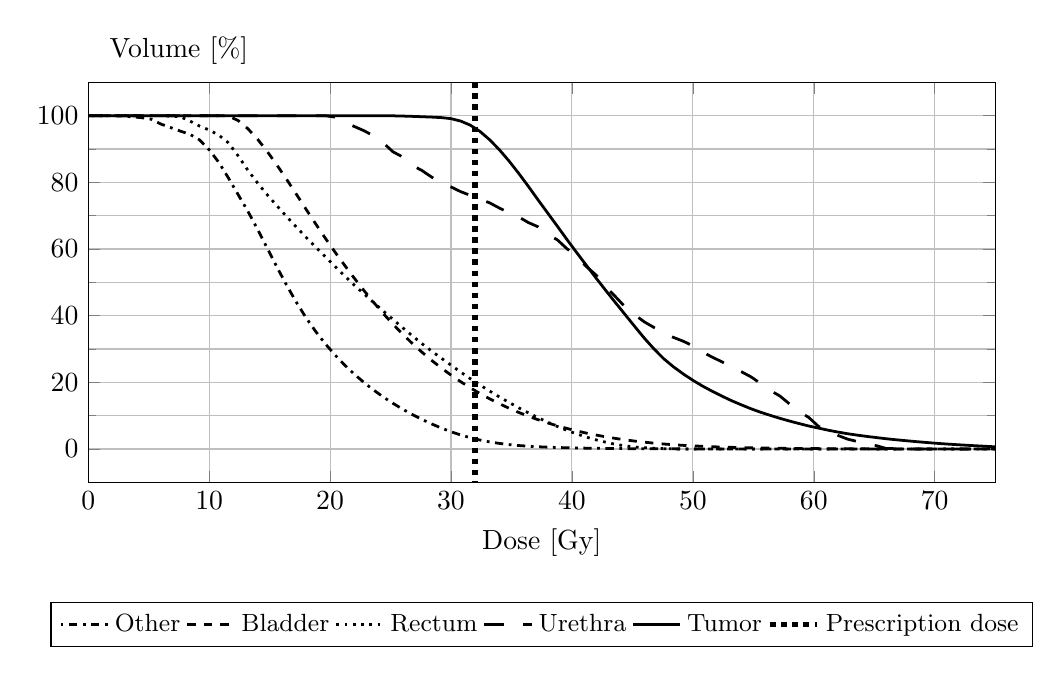
\begin{tikzpicture}
  \begin{axis}[
  	name=one,
  	width=0.95 \columnwidth,
  	height=2.0in, 
  	scale only axis,
  	xtick={0,10,...,80},
  	ytick={0,20,...,100},
  	minor ytick={10,30,...,90},
  	legend style={anchor=north,at={(0.5,-0.30)},font=\small},
  	legend columns=6,
    xmin=0,
    xmax=75,
  	ymax = 110,
  	ymin = -10,
    grid=both,
    y label style={at={(axis description cs:0.1,1.02)},anchor=south,rotate=270},
    ylabel = {Volume [\%]},
    xlabel = {Dose [Gy]}
  	]
\addplot [color=black,dash pattern=on 1pt off 2pt on 3pt off 2pt,line width=1.0pt]
	table[row sep=crcr]{-0.4 100.0 \\
0.4 100.0 \\
1.2000000000000002 100.0 \\
2.0 99.98287739703625 \\
2.8000000000000003 99.89388087384742 \\
3.6 99.66780099639195 \\
4.4 99.3960950212187 \\
5.200000000000001 98.94434538853442 \\
6.000000000000001 97.49907466172606 \\
6.800000000000001 96.45531359483411 \\
7.6000000000000005 95.39555776110176 \\
8.4 94.43371860898844 \\
9.200000000000001 92.75437062130442 \\
10.000000000000002 89.79308308358598 \\
10.8 85.99934995627072 \\
11.600000000000001 81.29586319963008 \\
12.4 76.31462116497269 \\
13.200000000000001 71.3547054861025 \\
14.000000000000002 65.95800963582172 \\
14.8 60.29781025490123 \\
15.600000000000001 54.63248434614727 \\
16.4 49.19733953711555 \\
17.2 44.105672092925495 \\
18.0 39.46965044257315 \\
18.8 35.32290460864599 \\
19.6 31.593458140362284 \\
20.4 28.25239742074132 \\
21.2 25.217800535004447 \\
22.0 22.475313205217986 \\
22.8 19.97059423634729 \\
23.6 17.695851306085498 \\
24.4 15.612020272341665 \\
25.2 13.71202652670562 \\
26.0 11.953730010386344 \\
26.8 10.351382470760848 \\
27.6 8.874532332498392 \\
28.4 7.526665634525728 \\
29.2 6.292300262785816 \\
30.0 5.18763604523238 \\
30.8 4.216774204132187 \\
31.6 3.3853539201020384 \\
32.4 2.688453726421817 \\
33.2 2.125458439751507 \\
34.0 1.6833466793941265 \\
34.8 1.3195682643319775 \\
35.6 1.0445813113453135 \\
36.4 0.8426986452637546 \\
37.2 0.6791624073764584 \\
38.0 0.5531523532300714 \\
38.800000000000004 0.45236481602429557 \\
39.6 0.3745441235124098 \\
40.4 0.3070790172241082 \\
41.2 0.25663398334288573 \\
42.0 0.21141800785179002 \\
42.800000000000004 0.17696774081095518 \\
43.6 0.1472338793769013 \\
44.4 0.11996075130290705 \\
45.2 0.10078753720577575 \\
46.0 0.08222950644865935 \\
46.800000000000004 0.06797775907164733 \\
47.6 0.05618674505469492 \\
48.4 0.0469589949544713 \\
49.2 0.03855148930760089 \\
50.0 0.03219459479411351 \\
50.800000000000004 0.026760475290648494 \\
51.6 0.022249130797205835 \\
52.4 0.018455500200447235 \\
53.2 0.015482114057041849 \\
54.0 0.013431502923658823 \\
54.800000000000004 0.010765708450260888 \\
55.6 0.008920158430216164 \\
56.4 0.0076897917501863484 \\
57.2 0.006869547296833137 \\
58.0 0.005946772286810776 \\
58.800000000000004 0.005126527833457566 \\
59.6 0.004921466720119263 \\
60.4 0.004101222266766053 \\
61.2 0.0035885694834202966 \\
62.0 0.003178447256743691 \\
62.800000000000004 0.0026657944733979345 \\
63.6 0.0023582028033904807 \\
64.4 0.0020506111333830268 \\
65.2 0.001845550020044724 \\
66.00000000000001 0.00153795835003727 \\
66.80000000000001 0.0014354277933681188 \\
67.60000000000001 0.0012303666800298162 \\
68.4 0.0011278361233606647 \\
69.2 0.0010253055666915134 \\
70.00000000000001 9.22775010022362E-4 \\
70.80000000000001 9.22775010022362E-4 \\
71.60000000000001 6.15183340014908E-4 \\
72.4 4.101222266766053E-4 \\
73.2 4.101222266766053E-4 \\
74.00000000000001 2.0506111333830264E-4 \\
74.80000000000001 2.0506111333830264E-4 \\
75.60000000000001 2.0506111333830264E-4 \\
76.4 2.0506111333830264E-4 \\
77.20000000000002 0.0 \\
78.00000000000001 0.0 \\
78.80000000000001 0.0 \\
	};
\addlegendentry{Other};

\addplot [color=black,dashed,line width=1.0pt]
	table[row sep=crcr]{-0.4 99.99999999999997 \\
0.4 99.99999999999997 \\
1.2000000000000002 99.99999999999997 \\
2.0 99.99999999999997 \\
2.8000000000000003 99.99999999999997 \\
3.6 99.99999999999997 \\
4.4 99.99999999999997 \\
5.200000000000001 99.99999999999997 \\
6.000000000000001 99.99999999999997 \\
6.800000000000001 99.99999999999997 \\
7.6000000000000005 99.99999999999997 \\
8.4 99.99999999999997 \\
9.200000000000001 99.99999999999997 \\
10.000000000000002 99.99999999999997 \\
10.8 99.99999999999997 \\
11.600000000000001 99.8921449992108 \\
12.4 98.53606566001997 \\
13.200000000000001 96.1080128373757 \\
14.000000000000002 92.97364129005102 \\
14.8 89.28684168990371 \\
15.600000000000001 85.22123428210658 \\
16.4 80.9491240069448 \\
17.2 76.51523123059924 \\
18.0 72.02083442942073 \\
18.8 67.60272531172726 \\
19.6 63.28326406060925 \\
20.4 59.125585310675014 \\
21.2 55.13626558636292 \\
22.0 51.27321513126743 \\
22.8 47.562740043142 \\
23.6 44.007470931761986 \\
24.4 40.642921029094545 \\
25.2 37.45330667648761 \\
26.0 34.483348240122055 \\
26.8 31.6646498658389 \\
27.6 29.048508444257376 \\
28.4 26.583627084758245 \\
29.2 24.317356763297727 \\
30.0 22.1734097963908 \\
30.8 20.19782185510601 \\
31.6 18.361656231914555 \\
32.4 16.64912926816436 \\
33.2 15.049718524754036 \\
34.0 13.587099489661703 \\
34.8 12.232335455358552 \\
35.6 10.980165202293891 \\
36.4 9.826642815804703 \\
37.2 8.795443783869102 \\
38.0 7.8300099963171474 \\
38.800000000000004 6.948755721576262 \\
39.6 6.1635187036355035 \\
40.4 5.432209186089336 \\
41.2 4.769295522702163 \\
42.0 4.185300152575367 \\
42.800000000000004 3.6565475877308358 \\
43.6 3.1817225232808966 \\
44.4 2.748987215236492 \\
45.2 2.3741253222496974 \\
46.0 2.0466144052191297 \\
46.800000000000004 1.7519861103803862 \\
47.6 1.5033934866101963 \\
48.4 1.2811069605934655 \\
49.2 1.0969642763192509 \\
50.0 0.9457042142368601 \\
50.800000000000004 0.8062818961435262 \\
51.6 0.6865891513652865 \\
52.4 0.5826800652391225 \\
53.2 0.5037617719787448 \\
54.0 0.4287893933813859 \\
54.800000000000004 0.36170884411006476 \\
55.6 0.3077813437154733 \\
56.4 0.2722681117483033 \\
57.2 0.22754774556742255 \\
58.0 0.18940390382490663 \\
58.800000000000004 0.16046719629610143 \\
59.6 0.13810701320566107 \\
60.4 0.11574683011522072 \\
61.2 0.10390908612616405 \\
62.0 0.07760298837270478 \\
62.800000000000004 0.06444993949597516 \\
63.6 0.055242805282264426 \\
64.4 0.043405061293207765 \\
65.2 0.03288262219182407 \\
66.00000000000001 0.03025201241647814 \\
66.80000000000001 0.022360183090440362 \\
67.60000000000001 0.017098963539748515 \\
68.4 0.01446835376440259 \\
69.2 0.010522439101383702 \\
70.00000000000001 0.007891829326037774 \\
70.80000000000001 0.006576524438364813 \\
71.60000000000001 0.005261219550691851 \\
72.4 0.0026306097753459254 \\
73.2 0.0013153048876729627 \\
74.00000000000001 0.0013153048876729627 \\
74.80000000000001 0.0 \\
75.60000000000001 0.0 \\
76.4 0.0 \\
77.20000000000002 0.0 \\
78.00000000000001 0.0 \\
78.80000000000001 0.0 \\
	};
\addlegendentry{Bladder};

\addplot [color=black,dotted,line width=1.0pt]
	table[row sep=crcr]{-0.4 100.0 \\
0.4 100.0 \\
1.2000000000000002 100.0 \\
2.0 100.0 \\
2.8000000000000003 100.0 \\
3.6 100.0 \\
4.4 100.0 \\
5.200000000000001 100.0 \\
6.000000000000001 100.0 \\
6.800000000000001 99.84689971931616 \\
7.6000000000000005 99.73207450880328 \\
8.4 98.40520540954326 \\
9.200000000000001 96.89546653057754 \\
10.000000000000002 95.70681296249045 \\
10.8 94.15879901335376 \\
11.600000000000001 91.84528366079783 \\
12.4 87.93697371778515 \\
13.200000000000001 83.65229225142468 \\
14.000000000000002 79.84392276941396 \\
14.8 76.29497320745088 \\
15.600000000000001 73.01394913668453 \\
16.4 69.75418899379093 \\
17.2 66.6390235604321 \\
18.0 63.5791443395424 \\
18.8 60.64046950752744 \\
19.6 57.71880581781067 \\
20.4 54.81840605596666 \\
21.2 51.95415497150634 \\
22.0 49.16858042017521 \\
22.8 46.555243684613416 \\
23.6 43.95041252020073 \\
24.4 41.41575231776813 \\
25.2 38.88959768648464 \\
26.0 36.395338947010295 \\
26.8 33.96912477672876 \\
27.6 31.615207961214598 \\
28.4 29.369737177851498 \\
29.2 27.251849961724933 \\
30.0 25.161605851832952 \\
30.8 23.084120098664627 \\
31.6 21.087437271412774 \\
32.4 19.199200476311983 \\
33.2 17.376881857616738 \\
34.0 15.631113379263418 \\
34.8 13.981032576337501 \\
35.6 12.360721272433445 \\
36.4 10.853108786254998 \\
37.2 9.388024155822064 \\
38.0 8.03563834311474 \\
38.800000000000004 6.757676277962066 \\
39.6 5.579654673811347 \\
40.4 4.507952709024411 \\
41.2 3.5723398826231185 \\
42.0 2.7409203027983327 \\
42.800000000000004 2.034957897422812 \\
43.6 1.4012928468146635 \\
44.4 0.9419920047631197 \\
45.2 0.5975163732244619 \\
46.0 0.3806243089223441 \\
46.800000000000004 0.21901845708939355 \\
47.6 0.1041932465765076 \\
48.4 0.042527855745513314 \\
49.2 0.012758356723653993 \\
50.0 0.0 \\
50.800000000000004 0.0 \\
51.6 0.0 \\
52.4 0.0 \\
53.2 0.0 \\
54.0 0.0 \\
54.800000000000004 0.0 \\
55.6 0.0 \\
56.4 0.0 \\
57.2 0.0 \\
58.0 0.0 \\
58.800000000000004 0.0 \\
59.6 0.0 \\
60.4 0.0 \\
61.2 0.0 \\
62.0 0.0 \\
62.800000000000004 0.0 \\
63.6 0.0 \\
64.4 0.0 \\
65.2 0.0 \\
66.00000000000001 0.0 \\
66.80000000000001 0.0 \\
67.60000000000001 0.0 \\
68.4 0.0 \\
69.2 0.0 \\
70.00000000000001 0.0 \\
70.80000000000001 0.0 \\
71.60000000000001 0.0 \\
72.4 0.0 \\
73.2 0.0 \\
74.00000000000001 0.0 \\
74.80000000000001 0.0 \\
75.60000000000001 0.0 \\
76.4 0.0 \\
77.20000000000002 0.0 \\
78.00000000000001 0.0 \\
78.80000000000001 0.0 \\
	};
	\addlegendentry{Rectum};

\addplot [color=black,dash pattern=on 7pt off 7pt,line width=1.0pt]
	table[row sep=crcr]{-0.4 99.99999999999999 \\
0.4 99.99999999999999 \\
1.2000000000000002 99.99999999999999 \\
2.0 99.99999999999999 \\
2.8000000000000003 99.99999999999999 \\
3.6 99.99999999999999 \\
4.4 99.99999999999999 \\
5.200000000000001 99.99999999999999 \\
6.000000000000001 99.99999999999999 \\
6.800000000000001 99.99999999999999 \\
7.6000000000000005 99.99999999999999 \\
8.4 99.99999999999999 \\
9.200000000000001 99.99999999999999 \\
10.000000000000002 99.99999999999999 \\
10.8 99.99999999999999 \\
11.600000000000001 99.99999999999999 \\
12.4 99.99999999999999 \\
13.200000000000001 99.99999999999999 \\
14.000000000000002 99.99999999999999 \\
14.8 99.99999999999999 \\
15.600000000000001 99.99999999999999 \\
16.4 99.99999999999999 \\
17.2 99.99999999999999 \\
18.0 99.99999999999999 \\
18.8 99.99999999999999 \\
19.6 99.99999999999999 \\
20.4 99.57805907172995 \\
21.2 98.17158931082982 \\
22.0 96.76511954992966 \\
22.8 95.49929676511954 \\
23.6 93.95218002812939 \\
24.4 91.84247538677918 \\
25.2 89.17018284106892 \\
26.0 87.62306610407877 \\
26.8 85.09142053445852 \\
27.6 83.54430379746837 \\
28.4 81.57524613220816 \\
29.2 79.88748241912799 \\
30.0 78.62165963431788 \\
30.8 77.21518987341773 \\
31.6 76.09001406469761 \\
32.4 74.96483825597751 \\
33.2 73.8396624472574 \\
34.0 72.29254571026725 \\
34.8 70.8860759493671 \\
35.6 69.62025316455697 \\
36.4 67.93248945147681 \\
37.2 66.66666666666669 \\
38.0 64.41631504922645 \\
38.800000000000004 62.72855133614629 \\
39.6 60.056258790436026 \\
40.4 57.805907172995795 \\
41.2 54.711673699015485 \\
42.0 52.180028129395225 \\
42.800000000000004 48.66385372714488 \\
43.6 45.71026722925458 \\
44.4 42.61603375527427 \\
45.2 40.22503516174403 \\
46.0 38.11533052039382 \\
46.800000000000004 36.42756680731365 \\
47.6 34.73980309423348 \\
48.4 33.473980309423354 \\
49.2 32.34880450070324 \\
50.0 30.942334739803094 \\
50.800000000000004 29.11392405063291 \\
51.6 27.566807313642755 \\
52.4 26.160337552742615 \\
53.2 24.613220815752456 \\
54.0 23.206751054852315 \\
54.800000000000004 21.65963431786216 \\
55.6 19.690576652601965 \\
56.4 17.580872011251756 \\
57.2 15.893108298171587 \\
58.0 13.502109704641349 \\
58.800000000000004 11.251758087201125 \\
59.6 9.423347398030941 \\
60.4 6.751054852320674 \\
61.2 5.9071729957805905 \\
62.0 4.0787623066104075 \\
62.800000000000004 2.9535864978902953 \\
63.6 2.250351617440225 \\
64.4 1.4064697609001406 \\
65.2 0.9845288326300984 \\
66.00000000000001 0.14064697609001406 \\
66.80000000000001 0.14064697609001406 \\
67.60000000000001 0.0 \\
68.4 0.0 \\
69.2 0.0 \\
70.00000000000001 0.0 \\
70.80000000000001 0.0 \\
71.60000000000001 0.0 \\
72.4 0.0 \\
73.2 0.0 \\
74.00000000000001 0.0 \\
74.80000000000001 0.0 \\
75.60000000000001 0.0 \\
76.4 0.0 \\
77.20000000000002 0.0 \\
78.00000000000001 0.0 \\
78.80000000000001 0.0 \\
	};
\addlegendentry{Urethra};

\addplot [color=black,solid,line width=1.0pt]
	table[row sep=crcr]{-0.4 100.00000000000003 \\
0.4 100.00000000000003 \\
1.2000000000000002 100.00000000000003 \\
2.0 100.00000000000003 \\
2.8000000000000003 100.00000000000003 \\
3.6 100.00000000000003 \\
4.4 100.00000000000003 \\
5.200000000000001 100.00000000000003 \\
6.000000000000001 100.00000000000003 \\
6.800000000000001 100.00000000000003 \\
7.6000000000000005 100.00000000000003 \\
8.4 100.00000000000003 \\
9.200000000000001 100.00000000000003 \\
10.000000000000002 100.00000000000003 \\
10.8 100.00000000000003 \\
11.600000000000001 100.00000000000003 \\
12.4 100.00000000000003 \\
13.200000000000001 100.00000000000003 \\
14.000000000000002 100.00000000000003 \\
14.8 100.00000000000003 \\
15.600000000000001 100.00000000000003 \\
16.4 100.00000000000003 \\
17.2 100.00000000000003 \\
18.0 100.00000000000003 \\
18.8 100.00000000000003 \\
19.6 100.00000000000003 \\
20.4 100.00000000000003 \\
21.2 100.00000000000003 \\
22.0 100.00000000000003 \\
22.8 100.00000000000003 \\
23.6 100.00000000000003 \\
24.4 99.99358639582934 \\
25.2 99.95510477080528 \\
26.0 99.88638758326233 \\
26.8 99.7947646665384 \\
27.6 99.6875658539714 \\
28.4 99.5730372080665 \\
29.2 99.42369185380649 \\
30.0 99.11125770777788 \\
30.8 98.38743666565883 \\
31.6 97.15235974822023 \\
32.4 95.26126274703829 \\
33.2 92.77095187048184 \\
34.0 89.77671495194379 \\
34.8 86.40041047066693 \\
35.6 82.69243103084943 \\
36.4 78.7828811742393 \\
37.2 74.73406448420879 \\
38.0 70.772289565066 \\
38.800000000000004 66.81143087509047 \\
39.6 62.79468220591333 \\
40.4 58.90803807848418 \\
41.2 55.072702784420436 \\
42.0 51.27035174037729 \\
42.800000000000004 47.555042467221895 \\
43.6 43.911199069111156 \\
44.4 40.315915816864106 \\
45.2 36.725213710453254 \\
46.0 33.19589895824743 \\
46.800000000000004 29.9762696645685 \\
47.6 27.052582391907865 \\
48.4 24.648397057071918 \\
49.2 22.53465636825083 \\
50.0 20.616072492051714 \\
50.800000000000004 18.886231824303895 \\
51.6 17.32222863582639 \\
52.4 15.87641900992276 \\
53.2 14.498410342394838 \\
54.0 13.266082112457966 \\
54.800000000000004 12.086895174220976 \\
55.6 11.028650486059572 \\
56.4 10.096845422977195 \\
57.2 9.205354443253347 \\
58.0 8.387161796908643 \\
58.800000000000004 7.619361754762101 \\
59.6 6.890959566806849 \\
60.4 6.265175045582401 \\
61.2 5.637558066023473 \\
62.0 5.081406961509213 \\
62.800000000000004 4.583894523698268 \\
63.6 4.1578479609319885 \\
64.4 3.7721154815242386 \\
65.2 3.4211997104715826 \\
66.00000000000001 3.0757813144223634 \\
66.80000000000001 2.7761743767351086 \\
67.60000000000001 2.5022218557305553 \\
68.4 2.238347855565634 \\
69.2 1.9918822095782596 \\
70.00000000000001 1.7564113135977568 \\
70.80000000000001 1.543846146798237 \\
71.60000000000001 1.3532704800124604 \\
72.4 1.180103167404231 \\
73.2 1.0151819173011551 \\
74.00000000000001 0.854841813034276 \\
74.80000000000001 0.6990828546035933 \\
75.60000000000001 0.5634809378521755 \\
76.4 0.43062770860247557 \\
77.20000000000002 0.3005231668544936 \\
78.00000000000001 0.18874320845129783 \\
78.80000000000001 0.09345537505840962 \\
	};
\addlegendentry{Tumor};
  \addplot [color=black,dotted,line width=2.0pt]
  	table[row sep=crcr]{32.0 110.0 \\
  	32.0 -10.0 \\
  	};
  	 \addlegendentry{Prescription dose};
  \addplot [color=black,dotted,line width=2.0pt]
  	table[row sep=crcr]{32.0 110.0 \\
  	32.0 -10.0 \\
  	};
\end{axis}

    
\end{tikzpicture} 
						\caption{50 seeds}
						\label{fig:lpswComparison50Seeds}
					\end{subfigure}
					\begin{subfigure}[t]{\textwidth}
						%\centering
						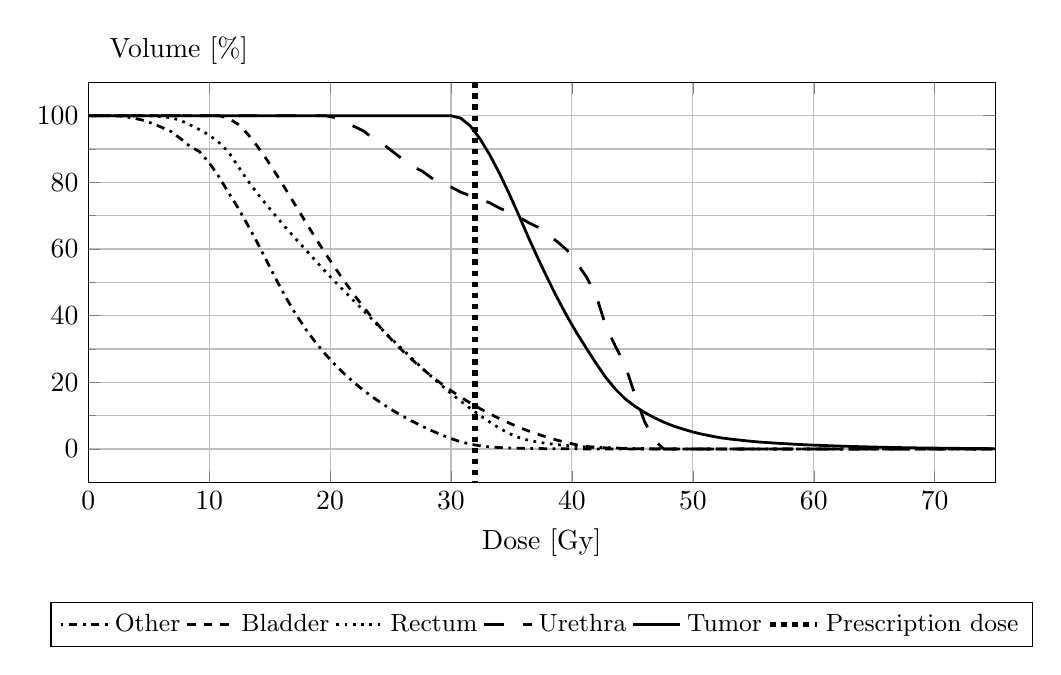
\begin{tikzpicture}
  \begin{axis}[
  	name=one,
  	width=0.95 \columnwidth,
  	height=2.0in, 
  	scale only axis,
  	xtick={0,10,...,80},
  	ytick={0,20,...,100},
  	minor ytick={10,30,...,90},
  	legend style={anchor=north,at={(0.5,-0.30)},font=\small},
  	legend columns=6,
    xmin=0,
    xmax=75,
  	ymax = 110,
  	ymin = -10,
    grid=both,
    y label style={at={(axis description cs:0.1,1.02)},anchor=south,rotate=270},
    ylabel = {Volume [\%]},
    xlabel = {Dose [Gy]}
  	]
    \addplot [color=black,dash pattern=on 1pt off 2pt on 3pt off 2pt,line width=1.0pt]
    	table[row sep=crcr]{-0.4 100.00000000000003 \\
    0.4 100.00000000000003 \\
    1.2000000000000002 100.00000000000003 \\
    2.0 99.99692408960745 \\
    2.8000000000000003 99.83687421884694 \\
    3.6 99.37220668887477 \\
    4.4 98.75784485313042 \\
    5.200000000000001 97.80472275281679 \\
    6.000000000000001 96.63587680363698 \\
    6.800000000000001 95.36398785630578 \\
    7.6000000000000005 93.22028337337144 \\
    8.4 90.84209198817621 \\
    9.200000000000001 89.22426565202638 \\
    10.000000000000002 85.90751147570903 \\
    10.8 81.73739722614401 \\
    11.600000000000001 76.95128065529195 \\
    12.4 72.28266386143639 \\
    13.200000000000001 67.16834765169621 \\
    14.000000000000002 61.81954453969514 \\
    14.8 56.149206261323194 \\
    15.600000000000001 50.497528505999554 \\
    16.4 45.132730659957076 \\
    17.2 40.23331805631171 \\
    18.0 35.87639351557076 \\
    18.8 31.985161808266195 \\
    19.6 28.49277314853263 \\
    20.4 25.33278787189038 \\
    21.2 22.483572075244968 \\
    22.0 19.884017672130504 \\
    22.8 17.535560087396863 \\
    23.6 15.371554595871512 \\
    24.4 13.391591076168769 \\
    25.2 11.562244635355949 \\
    26.0 9.872031874634095 \\
    26.8 8.31182759317189 \\
    27.6 6.860613069953379 \\
    28.4 5.507212497218864 \\
    29.2 4.269466155245299 \\
    30.0 3.1325071438018868 \\
    30.8 2.158058731433036 \\
    31.6 1.4481386128259313 \\
    32.4 0.9644004384197612 \\
    33.2 0.6398918920027354 \\
    34.0 0.43698433643897755 \\
    34.8 0.3066682661400708 \\
    35.6 0.22689965662586986 \\
    36.4 0.17276363371648923 \\
    37.2 0.1309312523774224 \\
    38.0 0.10119745191583078 \\
    38.800000000000004 0.07833318466433102 \\
    39.6 0.05905747953750611 \\
    40.4 0.045831064849418804 \\
    41.2 0.03424513570404 \\
    42.0 0.0254275259119818 \\
    42.800000000000004 0.019275705126824912 \\
    43.6 0.014456778845118683 \\
    44.4 0.01138086845254024 \\
    45.2 0.007997367020703952 \\
    46.0 0.006151820785156886 \\
    46.800000000000004 0.004921456628125509 \\
    47.6 0.003178440738997725 \\
    48.4 0.0024607283140627547 \\
    49.2 0.001640485542708503 \\
    50.0 6.151820785156887E-4 \\
    50.800000000000004 4.1012138567712576E-4 \\
    51.6 3.0759103925784433E-4 \\
    52.4 3.0759103925784433E-4 \\
    53.2 3.0759103925784433E-4 \\
    54.0 3.0759103925784433E-4 \\
    54.800000000000004 3.0759103925784433E-4 \\
    55.6 3.0759103925784433E-4 \\
    56.4 2.0506069283856288E-4 \\
    57.2 2.0506069283856288E-4 \\
    58.0 1.0253034641928144E-4 \\
    58.800000000000004 1.0253034641928144E-4 \\
    59.6 1.0253034641928144E-4 \\
    60.4 1.0253034641928144E-4 \\
    61.2 1.0253034641928144E-4 \\
    62.0 1.0253034641928144E-4 \\
    62.800000000000004 1.0253034641928144E-4 \\
    63.6 1.0253034641928144E-4 \\
    64.4 1.0253034641928144E-4 \\
    65.2 1.0253034641928144E-4 \\
    66.00000000000001 1.0253034641928144E-4 \\
    66.80000000000001 1.0253034641928144E-4 \\
    67.60000000000001 1.0253034641928144E-4 \\
    68.4 1.0253034641928144E-4 \\
    69.2 1.0253034641928144E-4 \\
    70.00000000000001 1.0253034641928144E-4 \\
    70.80000000000001 1.0253034641928144E-4 \\
    71.60000000000001 1.0253034641928144E-4 \\
    72.4 1.0253034641928144E-4 \\
    73.2 1.0253034641928144E-4 \\
    74.00000000000001 1.0253034641928144E-4 \\
    74.80000000000001 1.0253034641928144E-4 \\
    75.60000000000001 1.0253034641928144E-4 \\
    76.4 0.0 \\
    77.20000000000002 0.0 \\
    78.00000000000001 0.0 \\
    78.80000000000001 0.0 \\
    	};
    \addlegendentry{Other};
    
    \addplot [color=black,dashed,line width=1.0pt]
    	table[row sep=crcr]{-0.4 100.0 \\
    0.4 100.0 \\
    1.2000000000000002 100.0 \\
    2.0 100.0 \\
    2.8000000000000003 100.0 \\
    3.6 100.0 \\
    4.4 100.0 \\
    5.200000000000001 100.0 \\
    6.000000000000001 100.0 \\
    6.800000000000001 100.0 \\
    7.6000000000000005 100.0 \\
    8.4 100.0 \\
    9.200000000000001 100.0 \\
    10.000000000000002 100.0 \\
    10.8 100.0 \\
    11.600000000000001 99.2844741411059 \\
    12.4 97.38122796864313 \\
    13.200000000000001 94.46914294733519 \\
    14.000000000000002 90.76655968853579 \\
    14.8 86.65754721944546 \\
    15.600000000000001 82.16315041826695 \\
    16.4 77.50828642079234 \\
    17.2 72.73899089809018 \\
    18.0 67.98547903404008 \\
    18.8 63.267480401957165 \\
    19.6 58.767822381227965 \\
    20.4 54.42994686168253 \\
    21.2 50.23543957489346 \\
    22.0 46.21192192350186 \\
    22.8 42.43436628610512 \\
    23.6 38.837007418319565 \\
    24.4 35.489556479191876 \\
    25.2 32.35781554164255 \\
    26.0 29.435208081233235 \\
    26.8 26.724364707739255 \\
    27.6 24.177934445204404 \\
    28.4 21.80117851317936 \\
    29.2 19.594096911664128 \\
    30.0 17.51854579891619 \\
    30.8 15.594254748250647 \\
    31.6 13.79360235702636 \\
    32.4 12.12842636923239 \\
    33.2 10.573735992002947 \\
    34.0 9.134792444888726 \\
    34.8 7.802388593676015 \\
    35.6 6.566001999263429 \\
    36.4 5.425632661650971 \\
    37.2 4.416793812805809 \\
    38.0 3.481612037670332 \\
    38.800000000000004 2.629294470458252 \\
    39.6 1.9085073920134688 \\
    40.4 1.2482243384016416 \\
    41.2 0.7628768348503184 \\
    42.0 0.5182301257431473 \\
    42.800000000000004 0.33014152680591363 \\
    43.6 0.23017835534276848 \\
    44.4 0.16046719629610146 \\
    45.2 0.0986478665754722 \\
    46.0 0.0631346346083022 \\
    46.800000000000004 0.03945914663018888 \\
    47.6 0.027621402641132213 \\
    48.4 0.011837743989056664 \\
    49.2 0.0 \\
    50.0 0.0 \\
    50.800000000000004 0.0 \\
    51.6 0.0 \\
    52.4 0.0 \\
    53.2 0.0 \\
    54.0 0.0 \\
    54.800000000000004 0.0 \\
    55.6 0.0 \\
    56.4 0.0 \\
    57.2 0.0 \\
    58.0 0.0 \\
    58.800000000000004 0.0 \\
    59.6 0.0 \\
    60.4 0.0 \\
    61.2 0.0 \\
    62.0 0.0 \\
    62.800000000000004 0.0 \\
    63.6 0.0 \\
    64.4 0.0 \\
    65.2 0.0 \\
    66.00000000000001 0.0 \\
    66.80000000000001 0.0 \\
    67.60000000000001 0.0 \\
    68.4 0.0 \\
    69.2 0.0 \\
    70.00000000000001 0.0 \\
    70.80000000000001 0.0 \\
    71.60000000000001 0.0 \\
    72.4 0.0 \\
    73.2 0.0 \\
    74.00000000000001 0.0 \\
    74.80000000000001 0.0 \\
    75.60000000000001 0.0 \\
    76.4 0.0 \\
    77.20000000000002 0.0 \\
    78.00000000000001 0.0 \\
    78.80000000000001 0.0 \\
    	};
    \addlegendentry{Bladder};
    
    \addplot [color=black,dotted,line width=1.0pt]
    	table[row sep=crcr]{-0.4 100.0 \\
    0.4 100.0 \\
    1.2000000000000002 100.0 \\
    2.0 100.0 \\
    2.8000000000000003 100.0 \\
    3.6 100.0 \\
    4.4 100.0 \\
    5.200000000000001 100.0 \\
    6.000000000000001 99.73420090159055 \\
    6.800000000000001 99.41736837628648 \\
    7.6000000000000005 98.64336140171814 \\
    8.4 97.29735476737264 \\
    9.200000000000001 95.81100620906695 \\
    10.000000000000002 94.19920047631199 \\
    10.8 92.00688951263078 \\
    11.600000000000001 89.13200646423407 \\
    12.4 84.80054435655354 \\
    13.200000000000001 80.54988517478948 \\
    14.000000000000002 76.59266819766947 \\
    14.8 73.01820192225907 \\
    15.600000000000001 69.50540103767968 \\
    16.4 66.16058518329505 \\
    17.2 62.924215361061485 \\
    18.0 59.732499787360716 \\
    18.8 56.48762439397805 \\
    19.6 53.30654078421367 \\
    20.4 50.20200731479119 \\
    21.2 47.32287148081994 \\
    22.0 44.32465765076125 \\
    22.8 41.422131496129964 \\
    23.6 38.428170451645826 \\
    24.4 35.49374840520541 \\
    25.2 32.640129284681464 \\
    26.0 29.860933911712166 \\
    26.8 27.08386493153015 \\
    27.6 24.328059879220888 \\
    28.4 21.708343965297267 \\
    29.2 19.14604065663009 \\
    30.0 16.68793059453942 \\
    30.8 14.370162456408947 \\
    31.6 12.177851492727736 \\
    32.4 10.057837883813898 \\
    33.2 8.093050948371182 \\
    34.0 6.240962830654078 \\
    34.8 4.68019052479374 \\
    35.6 3.4468827081738542 \\
    36.4 2.6218423067108962 \\
    37.2 2.0477162541464664 \\
    38.0 1.6394488389895385 \\
    38.800000000000004 1.299225993025432 \\
    39.6 1.024921323466871 \\
    40.4 0.8101556519520288 \\
    41.2 0.5953899804371865 \\
    42.0 0.46993280598792214 \\
    42.800000000000004 0.3721187377732415 \\
    43.6 0.2913158118567662 \\
    44.4 0.2232712426639449 \\
    45.2 0.15735306625839926 \\
    46.0 0.11269881772561027 \\
    46.800000000000004 0.06166539083099431 \\
    47.6 0.03827507017096198 \\
    48.4 0.017011142298205325 \\
    49.2 0.010631963936378329 \\
    50.0 0.0 \\
    50.800000000000004 0.0 \\
    51.6 0.0 \\
    52.4 0.0 \\
    53.2 0.0 \\
    54.0 0.0 \\
    54.800000000000004 0.0 \\
    55.6 0.0 \\
    56.4 0.0 \\
    57.2 0.0 \\
    58.0 0.0 \\
    58.800000000000004 0.0 \\
    59.6 0.0 \\
    60.4 0.0 \\
    61.2 0.0 \\
    62.0 0.0 \\
    62.800000000000004 0.0 \\
    63.6 0.0 \\
    64.4 0.0 \\
    65.2 0.0 \\
    66.00000000000001 0.0 \\
    66.80000000000001 0.0 \\
    67.60000000000001 0.0 \\
    68.4 0.0 \\
    69.2 0.0 \\
    70.00000000000001 0.0 \\
    70.80000000000001 0.0 \\
    71.60000000000001 0.0 \\
    72.4 0.0 \\
    73.2 0.0 \\
    74.00000000000001 0.0 \\
    74.80000000000001 0.0 \\
    75.60000000000001 0.0 \\
    76.4 0.0 \\
    77.20000000000002 0.0 \\
    78.00000000000001 0.0 \\
    78.80000000000001 0.0 \\
    	};
    \addlegendentry{Rectum};
    
    \addplot [color=black,dash pattern=on 7pt off 7pt,line width=1.0pt]
    	table[row sep=crcr]{-0.4 99.99999999999997 \\
    0.4 99.99999999999997 \\
    1.2000000000000002 99.99999999999997 \\
    2.0 99.99999999999997 \\
    2.8000000000000003 99.99999999999997 \\
    3.6 99.99999999999997 \\
    4.4 99.99999999999997 \\
    5.200000000000001 99.99999999999997 \\
    6.000000000000001 99.99999999999997 \\
    6.800000000000001 99.99999999999997 \\
    7.6000000000000005 99.99999999999997 \\
    8.4 99.99999999999997 \\
    9.200000000000001 99.99999999999997 \\
    10.000000000000002 99.99999999999997 \\
    10.8 99.99999999999997 \\
    11.600000000000001 99.99999999999997 \\
    12.4 99.99999999999997 \\
    13.200000000000001 99.99999999999997 \\
    14.000000000000002 99.99999999999997 \\
    14.8 99.99999999999997 \\
    15.600000000000001 99.99999999999997 \\
    16.4 99.99999999999997 \\
    17.2 99.99999999999997 \\
    18.0 99.99999999999997 \\
    18.8 99.99999999999997 \\
    19.6 99.99999999999997 \\
    20.4 99.43741209563993 \\
    21.2 98.1715893108298 \\
    22.0 96.76511954992965 \\
    22.8 95.35864978902951 \\
    23.6 92.96765119549929 \\
    24.4 91.42053445850912 \\
    25.2 89.17018284106891 \\
    26.0 86.91983122362868 \\
    26.8 84.81012658227847 \\
    27.6 83.40365682137832 \\
    28.4 81.29395218002811 \\
    29.2 79.74683544303797 \\
    30.0 78.62165963431785 \\
    30.8 77.0745428973277 \\
    31.6 75.94936708860759 \\
    32.4 74.9648382559775 \\
    33.2 73.83966244725738 \\
    34.0 72.29254571026723 \\
    34.8 71.02672292545711 \\
    35.6 69.62025316455697 \\
    36.4 67.9324894514768 \\
    37.2 66.52601969057666 \\
    38.0 64.41631504922644 \\
    38.800000000000004 62.16596343178622 \\
    39.6 59.634317862165965 \\
    40.4 55.836849507735586 \\
    41.2 51.61744022503516 \\
    42.0 46.132208157524616 \\
    42.800000000000004 36.84950773558368 \\
    43.6 30.801687763713076 \\
    44.4 25.175808720112514 \\
    45.2 16.31504922644163 \\
    46.0 8.29817158931083 \\
    46.800000000000004 2.6722925457102673 \\
    47.6 0.0 \\
    48.4 0.0 \\
    49.2 0.0 \\
    50.0 0.0 \\
    50.800000000000004 0.0 \\
    51.6 0.0 \\
    52.4 0.0 \\
    53.2 0.0 \\
    54.0 0.0 \\
    54.800000000000004 0.0 \\
    55.6 0.0 \\
    56.4 0.0 \\
    57.2 0.0 \\
    58.0 0.0 \\
    58.800000000000004 0.0 \\
    59.6 0.0 \\
    60.4 0.0 \\
    61.2 0.0 \\
    62.0 0.0 \\
    62.800000000000004 0.0 \\
    63.6 0.0 \\
    64.4 0.0 \\
    65.2 0.0 \\
    66.00000000000001 0.0 \\
    66.80000000000001 0.0 \\
    67.60000000000001 0.0 \\
    68.4 0.0 \\
    69.2 0.0 \\
    70.00000000000001 0.0 \\
    70.80000000000001 0.0 \\
    71.60000000000001 0.0 \\
    72.4 0.0 \\
    73.2 0.0 \\
    74.00000000000001 0.0 \\
    74.80000000000001 0.0 \\
    75.60000000000001 0.0 \\
    76.4 0.0 \\
    77.20000000000002 0.0 \\
    78.00000000000001 0.0 \\
    78.80000000000001 0.0 \\
    	};
    \addlegendentry{Urethra};
    
    \addplot [color=black,solid,line width=1.0pt]
    	table[row sep=crcr]{-0.4 99.99999999999999 \\
    0.4 99.99999999999999 \\
    1.2000000000000002 99.99999999999999 \\
    2.0 99.99999999999999 \\
    2.8000000000000003 99.99999999999999 \\
    3.6 99.99999999999999 \\
    4.4 99.99999999999999 \\
    5.200000000000001 99.99999999999999 \\
    6.000000000000001 99.99999999999999 \\
    6.800000000000001 99.99999999999999 \\
    7.6000000000000005 99.99999999999999 \\
    8.4 99.99999999999999 \\
    9.200000000000001 99.99999999999999 \\
    10.000000000000002 99.99999999999999 \\
    10.8 99.99999999999999 \\
    11.600000000000001 99.99999999999999 \\
    12.4 99.99999999999999 \\
    13.200000000000001 99.99999999999999 \\
    14.000000000000002 99.99999999999999 \\
    14.8 99.99999999999999 \\
    15.600000000000001 99.99999999999999 \\
    16.4 99.99999999999999 \\
    17.2 99.99999999999999 \\
    18.0 99.99999999999999 \\
    18.8 99.99999999999999 \\
    19.6 99.99999999999999 \\
    20.4 99.99999999999999 \\
    21.2 99.99999999999999 \\
    22.0 99.99999999999999 \\
    22.8 99.99999999999999 \\
    23.6 99.99999999999999 \\
    24.4 99.99999999999999 \\
    25.2 99.99999999999999 \\
    26.0 99.99999999999999 \\
    26.8 99.99999999999999 \\
    27.6 99.99999999999999 \\
    28.4 99.99999999999999 \\
    29.2 99.99999999999999 \\
    30.0 99.97380236140093 \\
    30.8 99.26646611922635 \\
    31.6 96.89783824313216 \\
    32.4 93.06214260549066 \\
    33.2 88.26616800816643 \\
    34.0 82.7664706360606 \\
    34.8 76.67597134520358 \\
    35.6 70.18347380687824 \\
    36.4 63.48771872769814 \\
    37.2 57.1388565182435 \\
    38.0 51.0510673279312 \\
    38.800000000000004 45.22073768936828 \\
    39.6 39.809570268390296 \\
    40.4 34.81124149705954 \\
    41.2 30.195036902535747 \\
    42.0 25.683622862408196 \\
    42.800000000000004 21.47845018383515 \\
    43.6 17.930025203935067 \\
    44.4 15.038347922707931 \\
    45.2 12.842263114628219 \\
    46.0 10.976810573005592 \\
    46.800000000000004 9.411275824999775 \\
    47.6 8.042675049911018 \\
    48.4 6.894495785793653 \\
    49.2 5.9640279321029475 \\
    50.0 5.113959727905905 \\
    50.800000000000004 4.411140319972538 \\
    51.6 3.8347922707932462 \\
    52.4 3.310839498812072 \\
    53.2 2.941362457880521 \\
    54.0 2.62789416154006 \\
    54.800000000000004 2.3180393325925723 \\
    55.6 2.0678067156291497 \\
    56.4 1.870872742712088 \\
    57.2 1.687489272518677 \\
    58.0 1.519463038745404 \\
    58.800000000000004 1.3631805739992953 \\
    59.6 1.223158712521568 \\
    60.4 1.1057210222499254 \\
    61.2 1.0036405683984209 \\
    62.0 0.896139913457456 \\
    62.800000000000004 0.8021897612401421 \\
    63.6 0.7217901117464792 \\
    64.4 0.6441005627975466 \\
    65.2 0.5655076470003705 \\
    66.00000000000001 0.5049820681680625 \\
    66.80000000000001 0.448069956728728 \\
    67.60000000000001 0.3902544784411502 \\
    68.4 0.34418276918073665 \\
    69.2 0.3044346278580269 \\
    70.00000000000001 0.27552688871423797 \\
    70.80000000000001 0.24390904902571886 \\
    71.60000000000001 0.20867774194422614 \\
    72.4 0.18067336964868067 \\
    73.2 0.15357236420137857 \\
    74.00000000000001 0.12556799190583307 \\
    74.80000000000001 0.10117708700326117 \\
    75.60000000000001 0.08310975003839309 \\
    76.4 0.06142894568055142 \\
    77.20000000000002 0.04516834241217016 \\
    78.00000000000001 0.03161783968851911 \\
    78.80000000000001 0.015357236420137855 \\
    	};
    \addlegendentry{Tumor};
      \addplot [color=black,dotted,line width=2.0pt]
      	table[row sep=crcr]{32.0 110.0 \\
      	32.0 -10.0 \\
      	};
      	\addlegendentry{Prescription dose};
\end{axis}

    
\end{tikzpicture} 
						\caption{100 seeds}
						\label{fig:lpswComparison10Seeds}
					\end{subfigure}
			\caption{Final dose volume histograms with different numbers of seeds used for optimization}
			\label{fig:lpswComparison}
		\end{figure}
		
	\subsubsection{Discussion}
		The values for coverage and conformality index (CI) listed in Table \ref{table:lpswTable} indicate the conflicting multicriteria nature of the problem since one comes at another's cost. Therefore, the balancing of goals by relaxing dose constraints seems to be a reasonable approach to this problem.
			
		Improved treatment plans can be achieved by raising the number of seeds for the optimization process as demonstrated in the last two rows of Table \ref{table:lpswTable} and the corresponding dose volume histograms (Figure \ref{fig:lpswComparison}). The increased quality of a treatment plan comes at the cost of more computational complexity and therefore a longer computation time. 

\section{Classification}
While using computer aided systems to create treatment plans, this involves time-consuming calculations during optimizations (as seen in this project). Therefore, a classification attempt is proposed, using prior knowledge to reduce the amount of time taken to process.

\subsection{General Idea and Application}
When classifying, you search for similarities or analogies in your given set of data. These provide a basis for a comparison among previously created optimizations. The former result being the most similar (or closest with respect to the comparison) can be taken as a starting point for the next iteration.

In treatment planning, there are several steps to be executed when trying to classify. First, the body to be treated ("treated body") needs to be analyzed (i.e. measured in various variables). Second, these measurements build a formula providing a norm (like the euclidian norm), which then can be used to compare the bodies. Afterwards, the body with the smallest distance to the treated body is taken. If it has an optimization result stored ("stored body), this will be used during the next iteration. This aims at lower runtimes for at least an equal coverage.

\subsection{Parameters and Influences}
In table \ref{tbl:classification_parameters}, the various parameters measured in order to compare are displayed. Further on, their influence in the norm is shown. Additionally, in table \ref{tbl:classification_type_weights}, the weighted influence of the five different body types are presented.
\begin{table}
\centering
\caption{Parameters and Influences in classification}
\begin{tabular}[htbp]{l | c | c}
\textbf{Parameter} & \textbf{Influence Type} & \textbf{Weight} \\ \hline
volume size  & relative & 0.1\\ \hline
volume center & relative & 0.2 \\ \hline
distance tumor-center & absolute & 0.2\\ \hline
closest distance & absolute & 0.5
\end{tabular}
\label{tbl:classification_parameters}
\end{table}

\begin{description}
\item[Volume Size]~\\
The plain count of all voxels respective to the different body types. As the body is given as an equidistant 3D-array, it's comparable without calculation of the real volume.
\item[Volume Center]~\\ The center of the volume of each body type, with respect to the coordinates within the 3D-array. For calculation, all coordinates of the body type's voxels are summed up and divided by the volume size.
\item[Distance Tumor-Center]~\\ The distance between the center of the tumor center and the center of the other body type volumes, calculated by a simple substraction.
\item[Closest Distance]~\\ The closest distance between two volumes in units, corresponding to the 3D-array's distance inbetween the voxels.
\end{description}

The four parameters descripted above are calculated in a measuring algorithm, detailed further in section \ref{classification:algorithm}. They contain two types of influence onto the norm: textit{relative} and \textit{absolute}. \textit{relative} depicts a comparison with respect to the treated body's values of the same parameter. For example, the tumor volume size of the stored body will be divided by the tumor volume size of the treated body. In constrast, the \textit{absolute} comparison omits the division completely. This is due to division by 0, when the tumor overlaps with other body type volumes. \\

They each share a weight parameter, which sums up to 1 in total. The values shown in table \ref{tbl:classification_parameters} represent a multiplication factor within the norm. The norm itself is a sum of the different parameters multiplied with their weight, corresponding to the smallest error between the stored and treated bodies. The weights correspond to a simple consideration about how much each parameter should influence the the classification. To allow for small to medium deviations within the three first parameters (volume size, volume center and distance tumor-center), they have been chosen small. This enables a few transformations (i.e. translation of single/all volumes) of the body volumes resulting in a similar classification. Therefore, the weight for closest distance has been chosen larger, to prevent extreme transformations to distort the result. \\

Additionally to the weights of the various weights of the measurement parameters, it's possible to change the influence of the different body types (compare table \ref{tbl:classification_type_weights}). This leads to a more detailed and precise representation of the aims during the treatment planning. In this case, a high focus has been set upon not damaging the spine and the pancreas whilst treating the tumor properly. 

\begin{table}
\centering
\caption{Influences of Body Types}
\begin{tabular}[htbp]{c | c | c | c | c}
\textbf{normal} & \textbf{spine} & \textbf{liver} & \textbf{pancreas} & \textbf{tumor} \\ \hline
1 & 5 & 0.5 & 5 & 3
\end{tabular}
\label{tbl:classification_type_weights}
\end{table}

\subsection{Algorithm and Performance}\label{classification:algorithm}
The algorithm is shown in algorithm \ref{alg:classification}. It consists of a main loop, iterating through the stored body

\begin{algorithm}[H]
\label{alg:classification}
\ForAll{$voxels\ in\ body$}{
	$count\ body\_type;$ \\
	$sum\ up\ coordinates;$\\
	\If{$body\_type == tumor$}{
		$store\ coordinate\ for\ later\ usage;$
	}
}
$volumeCenter = coordinates / body\_type;$ \\
$centerDistance = euclid\_norm (tumorCenter, volumeCenter);$ \\
\ForAll{$voxels\ in\ body$}{
	\ForAll{$voxels\ stored\ in\ tumor$}{
		$calculated\ distance (voxel, tumor);$\\
		\If{distance $\textless$ closestDistance}{
			$update\ closestDistance;$
		}
	}
}
\caption{Measurement algorithm in pseudo code}
\end{algorithm}




\newpage
\bibliographystyle{plain}
\bibliography{lit}

\end{document}
